\chapter{Implementasi dan Pengujian Perangkat Lunak}
\label{chap:Implementasi dan Pengujian Perangkat Lunak}

\section{Implementasi Perangkat Lunak}

\subsection{Lingkungan Perangkat Kerat}

Perangkat keras yang digunakan dalam membangun perangkat lunak reduksi data adalah sebuah PC dengan spesifikasi berikut:

\begin{itemize}
\item \textit{Processor}: Intel i7 4790K @4.00 GHz

\item RAM: 16 GB DDR3

\item VGA: NVIDIA GeForce GTX 750TI 2GB

\item \textit{Harddisk}: 1TB + 256GB SSD 

\end{itemize}

\subsection{Lingkungan Perangkat Lunak}

linkungan perangkat lunak yang digunakan untuk membangun perangkat lunak adalah sebagai berikut:

\begin{itemize}

\item Sistem Operasi: Ubuntu 18.04.2 LTS

\item Bahasa Pemrograman: Scala

\item IDE: InteliJ IDE 2018

\item Versi Java: JDK 1.8.0\_181

\item Versi Scala: Scala 2.11.12

\item Versi SBT: SBT 1.2.8

\item Library Dependency:

\begin{itemize}
\item org.apache.spark:spark-core 2.1.0

\item org.scala-lang:scala-library 2.11.12
\end{itemize}

\end{itemize}


\subsection{\textit{User Interface}}

Implementasi rancangan tampilan antarmuka pada perangkat lunak ini menggunakan html, css, dan php. Berikut adalah tampilan setiap halaman:

\begin{enumerate}
\item Implementasi antarmuka untuk menu \textit{Submit} dapat dilihat pada Gambar ~\ref{fig:menusubmit}.

\begin{figure}[H]
    \centering  
    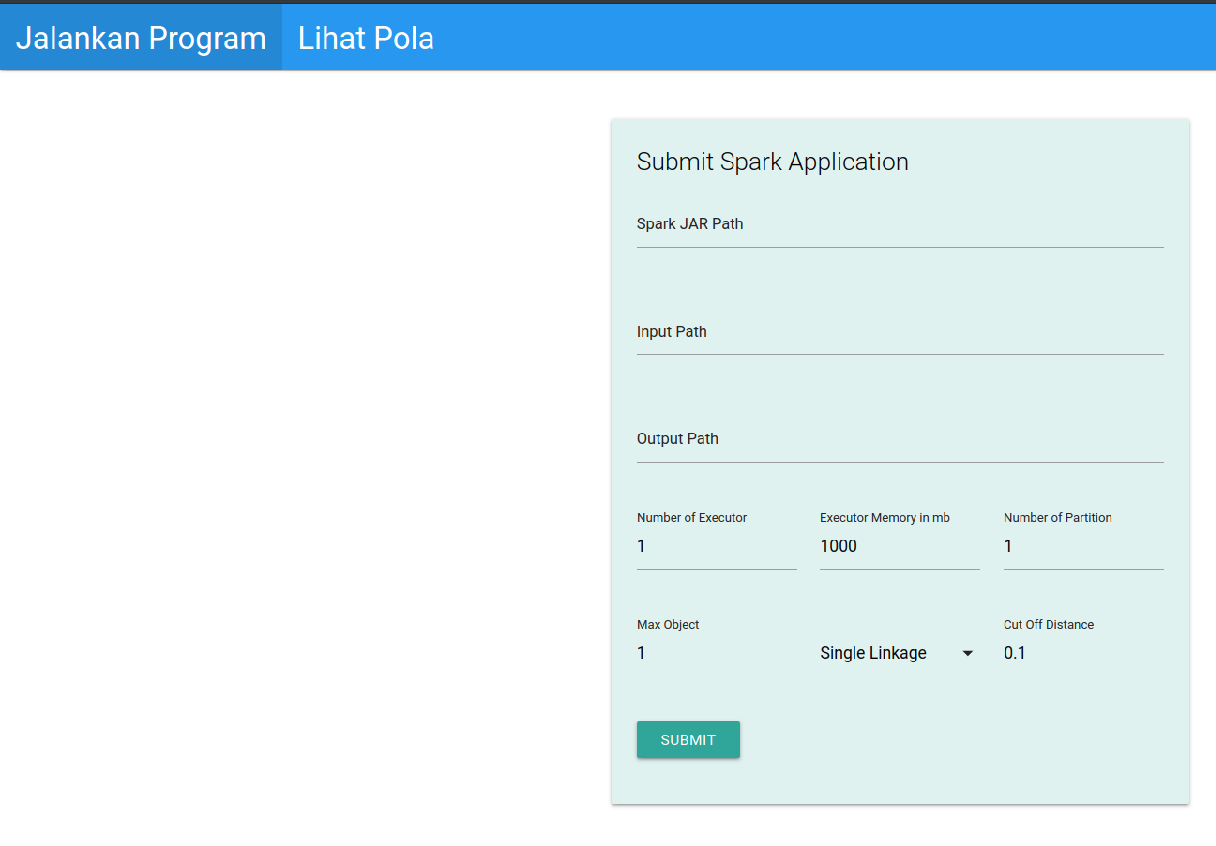
\includegraphics[scale=0.3]{menusubmit}  
    \caption[Tampilan menu \textit{Submit}]{Tampilan menu \textit{submit}} 
    \label{fig:menusubmit} 
\end{figure}

\item Implementasi antarmuka untuk menu \textit{Data} dapat dilihat pada Gambar ~\ref{fig:menudata}.

\begin{figure}[H]
    \centering  
    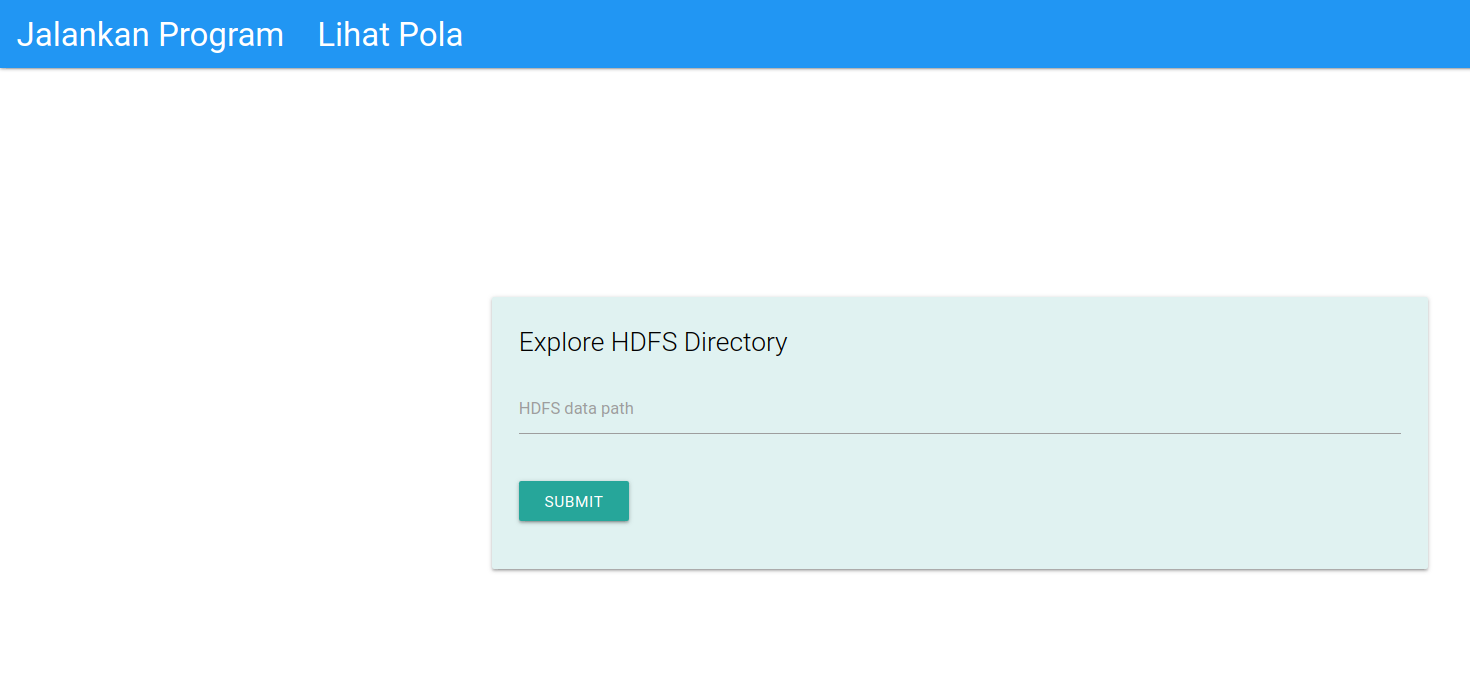
\includegraphics[scale=0.3]{menudata}  
    \caption[Tampilan menu \textit{Data}]{Tampilan menu \textit{Data}} 
    \label{fig:menudata} 
\end{figure}

\item Implementasi antarmuka sesudah melakukan \textit{submit} dapat dilihat pada Gambar ~\ref{fig:menuresult}.

\begin{figure}[H]
    \centering  
    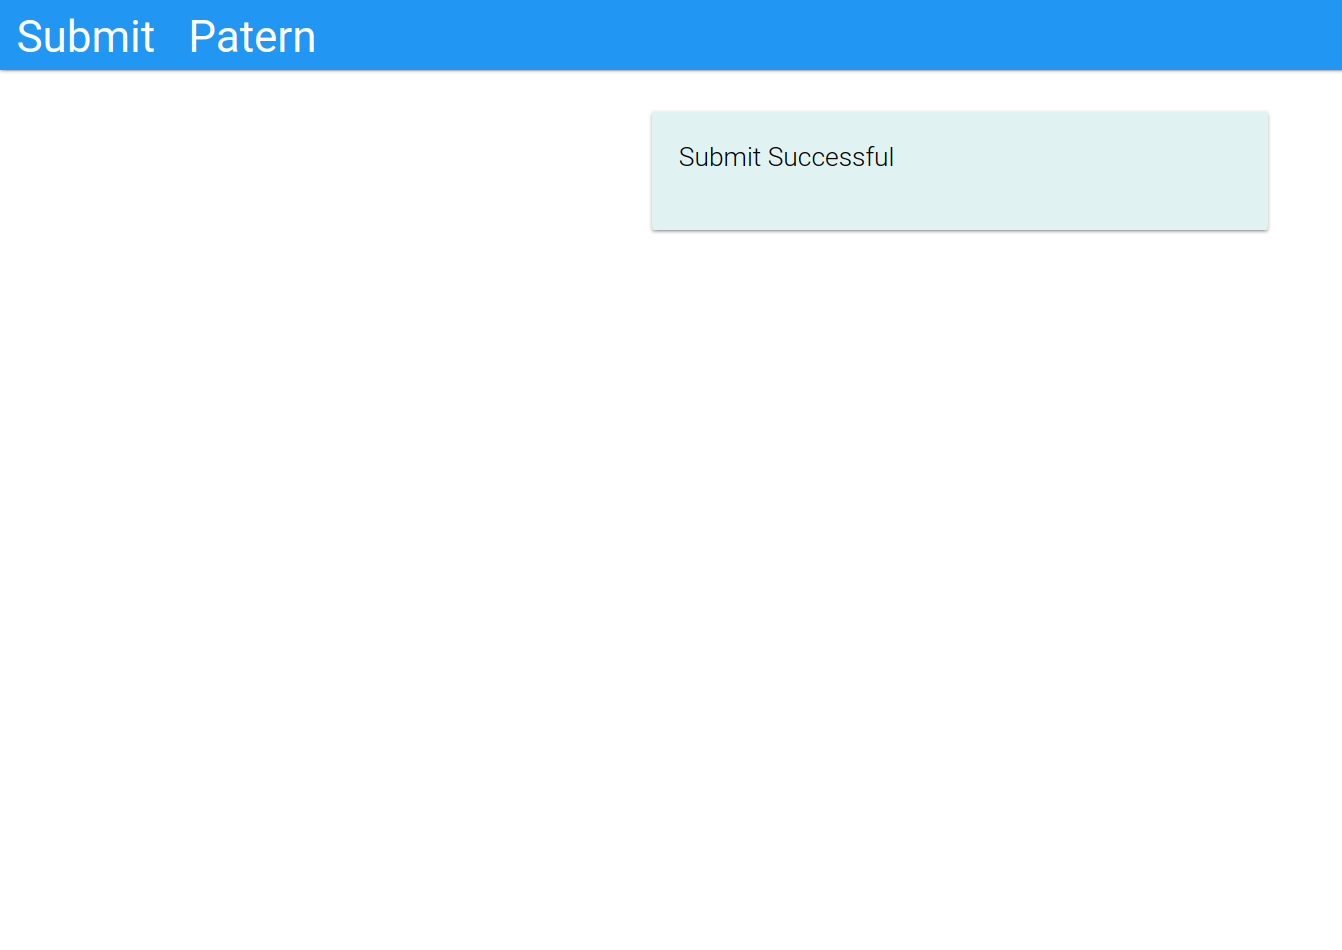
\includegraphics[scale=0.3]{menuresult}  
    \caption[Tampilan halaman sesudah \textit{submit}]{Tampilan halaman sesudah \textit{submit}} 
    \label{fig:menuresult} 
\end{figure}

\item Implementasi antarmuka  halaman \textit{list} dapat dilihat pada Gambar ~\ref{fig:menulist}.

\begin{figure}[H]
    \centering  
    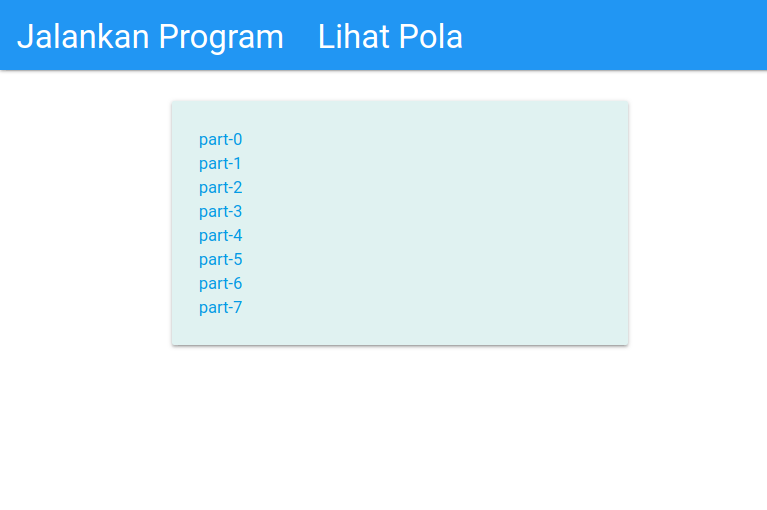
\includegraphics[scale=0.5]{menulist}  
    \caption[Tampilan halaman \textit{list}]{Tampilan halaman \textit{list}} 
    \label{fig:menulist} 
\end{figure}

\item Implementasi antarmuka  halaman \textit{data} dapat dilihat pada Gambar ~\ref{fig:menudata2}.

\begin{figure}[H]
    \centering  
    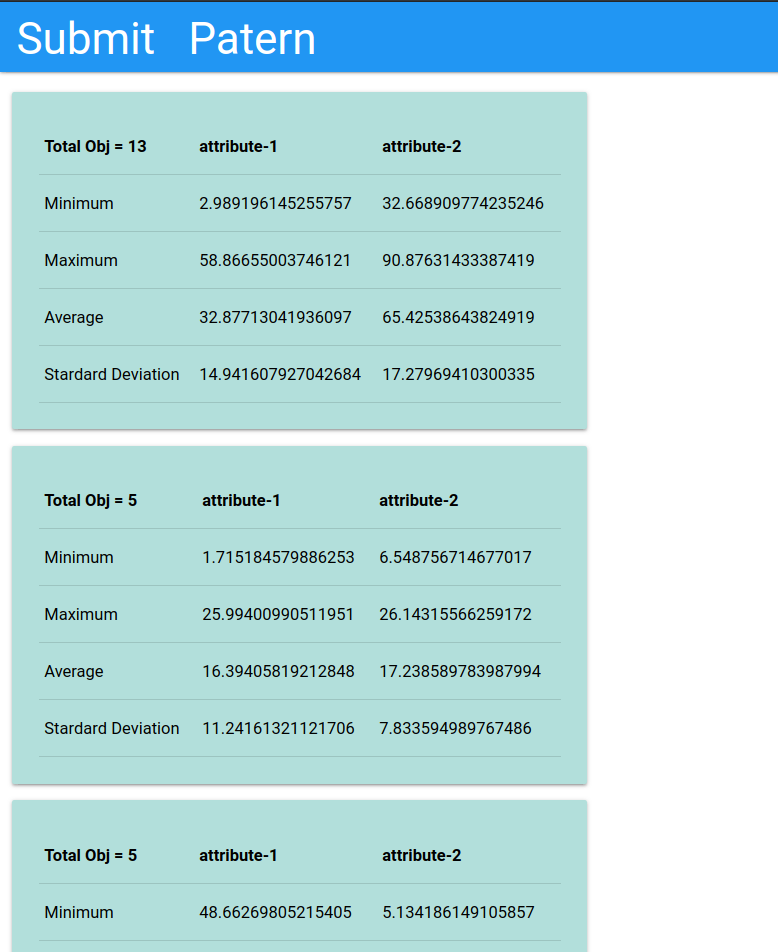
\includegraphics[scale=0.5]{menudata2}  
    \caption[Tampilan halaman data]{Tampilan halaman data} 
    \label{fig:menudata2} 
\end{figure}

\end{enumerate}

\section{Pengujian Fungsional Perangkat Lunak}

Perangkat lunak yang dibangun telah diuji untuk membuktikan kebenaran dan fungsionalitas dari perangkat lunak. Program akan dieksekusi dan kemudian dianalisis apakah hasil yang diberikan sesuai dengan yang diinginkan. Pengujian dilakukan dengan menggunakan data berukuran kecil beserta parameter-parameter yang telah ditentukan terhadap perangkat lunak.

\begin{itemize}

\item Pada percobaan pertama, digunakan metode \textit{single linkage} dengan jumlah partisi = 1, jumlah objek maksimum = 4, dan nilai \textit{cut-off distance} = 0.8. Berikut adalah data yang digunakan untuk pengujian:

\begin{verbatim}
4.0,5.0
3.0,7.0
4.0,3.0
10.0,7.0
10.0,10.0
\end{verbatim}

Hasil dari percobaan pertama adalah sebagai berikut:

\begin{verbatim}
3
3.0,3.0
4.0,7.0
3.6666666666666665,5.0
0.5773502691896258,2.0
1
10.0,7.0
10.0,7.0
10.0,7.0
0.0,0.0
1
10.0,10.0
10.0,10.0
10.0,10.0
0.0,0.0
\end{verbatim}

Perangkat lunak sudah dapat menghasilkan pola-pola dengan jumlah objek, nilai maksimum, minimum, rata-rata, dan standar deviasi. Nilai-nilai pada pola yang dihasilkan sudah akurat dengan apa yang diharapkan.

\item Pada percobaan kedua, akan digunakan metode \textit{complete linkage} dengan jumlah partisi = 1, jumlah objek maksimum = 4, dan nilai \textit{cut-off distance} = 0.8. Berikut adalah data yang digunakan untuk pengujian:

\begin{verbatim}
4.0,5.0
3.0,7.0
4.0,3.0
10.0,7.0
10.0,10.0
\end{verbatim}

Hasil dari percobaan kedua adalah sebagai berikut:

\begin{verbatim}
3
3.0,3.0
4.0,7.0
3.6666666666666665,5.0
0.5773502691896258,2.0
1
10.0,7.0
10.0,7.0
10.0,7.0
0.0,0.0
1
10.0,10.0
10.0,10.0
10.0,10.0
0.0,0.0
\end{verbatim}

Perangkat lunak sudah dapat menghasilkan pola-pola dengan jumlah objek, nilai maksimum, minimum, rata-rata, dan standar deviasi. Nilai-nilai pada pola yang dihasilkan sudah akurat dengan apa yang diharapkan.

\item Pada percobaan ketiga, akan digunakan metode \textit{centroid linkage} dengan jumlah partisi = 1, jumlah objek maksimum = 4, dan nilai \textit{cut-off distance} = 0.8. Berikut adalah data yang digunakan untuk pengujian:

\begin{verbatim}
4.0,5.0
3.0,7.0
4.0,3.0
10.0,7.0
10.0,10.0
\end{verbatim}

Hasil dari percobaan ketiga adalah sebagai berikut:

Perangkat lunak sudah dapat menghasilkan pola-pola dengan jumlah objek, nilai maksimum, minimum, rata-rata, dan standar deviasi. Nilai-nilai pada pola yang dihasilkan sudah akurat dengan apa yang diharapkan.

\begin{verbatim}
3
3.0,3.0
4.0,7.0
3.6666666666666665,5.0
0.5773502691896258,2.0
1
10.0,7.0
10.0,7.0
10.0,7.0
0.0,0.0
1
10.0,10.0
10.0,10.0
10.0,10.0
0.0,0.0
\end{verbatim}

 
\end{itemize}
Berdasarkan ketiga hasil percobaan yang didapat, dapat disimpulkan bahwa perangkat lunak sudah dapat melakukan proses reduksi data menggunakan algoritma \textit{Agglomerative Clustering} berdasarkan metode yang dipilih dengan benar. Pola yang dihasilkan oleh perangkat lunak sudah dapat menghasilkan jumlah objek, nilai maksimum, minimum, rata-rata, dan standar deviasi.

\section{Hasil Eksperimen Perangkat Lunak}

Selain menguji fungsionalitas perangkat lunak yang dibangun, diuji pula performa dari perangkat lunak Spark dan Hadoop. Kedua perangkat lunak kemudian dibandingkan hasil eksekusi waktunya. Karena perangkat lunak Hadoop tidak dapat menghitung standar deviasi, maka perangkat lunak Hadoop akan dibandingkan dengan perangkat lunak Spark yang tidak menghitung standar deviasi dan yang menghitung standar deviasi. Data yang digunakan pada percobaan merupakan data yang dihasilkan secara acak dengan ukuran yang berbeda-beda. Data-data tersebut memiliki dua atribut bilangan pecahan yang dipisahkan dengan tanda koma. Jumlah objek pada setiap ukuran data dapat dilihat pada Tabel ~\ref{tab:exdata}.\\

\begin{table}[H] 
	\centering 
	\caption{Tabel data yang digunakan pada eksperimen}
	\label{tab:exdata}
	\begin{tabular}{|p{2cm}|p{3cm}|p{4cm}|}
\hline
Ukuran Data & Jumlah Objek  & Jumlah Block\\
\hline
1 GB & 36000000 & 40 \\
\hline
2 GB & 64000000 & 70 \\
\hline
3 GB & 81000000 & 89 \\
\hline
5 GB & 144000000 & 157 \\
\hline
10 GB & 256000000 & 279 \\
\hline
15 GB & 400000000 & 435 \\
\hline
20 GB & 529000000 & 576 \\
\hline
	\end{tabular} 
\end{table}



Berikut adalah spesifikasi perangkat keras yang digunakan:

\begin{itemize}

\item \textit{Processor}: Intel core i5 8500 @3.00 GHz, 6 \textit{core}

\item RAM: 8GB

\item \textit{Harddisk}: 500GB

\item Sistem Operasi: Ubuntu 18.0.4

\end{itemize}







%1111111111GBBBBBBBBBBBBBBBBB

Percobaan ini menguji waktu eksekusi Spark dan Hadoop berdasarkan jumlah partisi yang berbeda. Percobaan ini menggunakan 1 komputer sebagai komputer \textit{master} dan 10 komputer lainya sebagai \textit{worker} dengan setiap \textit{worker} munggunakan 1 core. Ukuran data yang digunakan adalah 1 GB. Metode yang digunakan adalah metode \textit{single linkage}dengan nilai \textit{cut-off distance} adalah 0,8 dan jumlah objek maksimum untuk setiap \textit{dendrogram} adalah 30. Tabel~\ref{tab:spark1} berikut adalah hasil dari eksperimen:

\begin{table}[H] 
	\centering 
	\caption{Percobaan Jumlah Partisi Hadoop dan Spark dengan Ukuran Data 1 GB}
	\label{tab:spark1}
	\begin{tabular}{|p{1.1cm}|p{1.1cm}|p{2.5cm}|p{2.5cm}|p{2.5cm}|p{2cm}|p{1.5cm}|p{1.5cm}|}
\hline
Ukuran Data (GB) & Jumlah Partisi &  Waktu eksekusi Spark Tanpa standar Deviasi (Detik) & Waktu Eksekusi Spark (Detik) & Waktu Eksekusi Hadoop (Detik) & Hasil Reduksi Spark Tanpa standar Deviasi (GB) & Hasil Reduksi Spark (GB)  & Hasil Reduksi Hadoop (GB)\\ 
\hline
1 & 10 & 319 & 304 & 214 & 0.54 & 0.67 & 0.57 \\
\hline
1 & 30 & 131 & 124 & 216 & 0.54 & 0.67 & 0.57 \\
\hline
1 & 50 & 101 & 89 & 230 & 0.54 & 0.67 & 0.57 \\
\hline
1 & 100 & 62 & 63 & 303 & 0.54 & 0.67 & 0.57 \\
\hline
1 & 150 & 56 & 56 & 313 & 0.54 & 0.67 & 0.57 \\
\hline

\hline

	\end{tabular} 
\end{table}




\def\scl{1}

\def\leg{} 
\def\std{none}
\def\ymin{}
\def\ymax{}

\begin{minipage}[c]{0.9\textwidth}
	\begin{figure}[H]
		\centering
		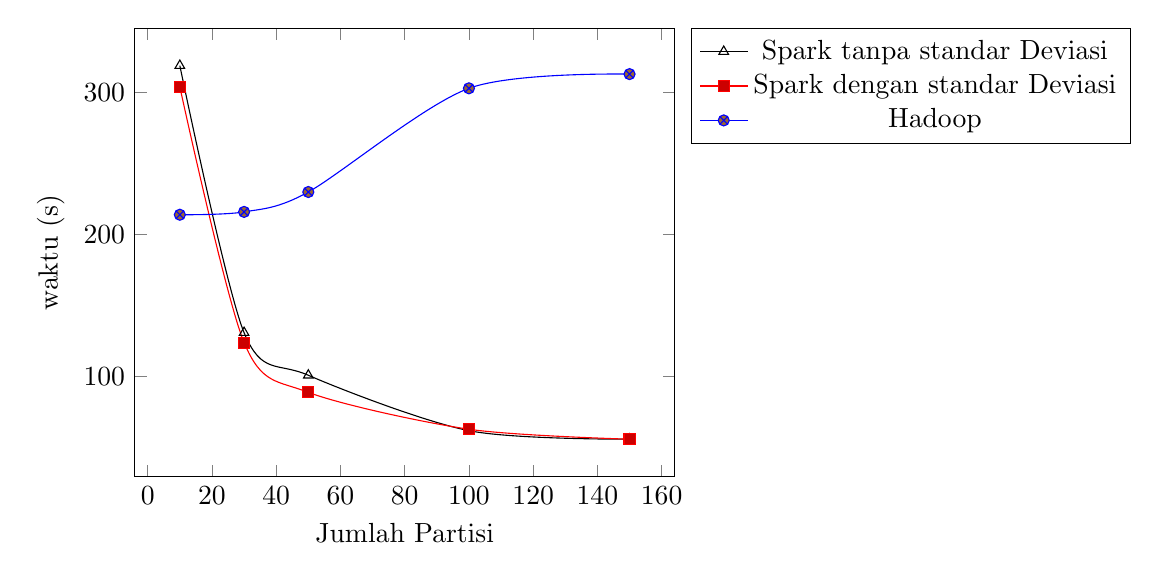
\begin{tikzpicture}[scale=\scl]
		\begin{axis}[\ymin,\ymax,xlabel= Jumlah Partisi,ylabel= waktu (s), xticklabel style={/pgf/number format/.cd, fixed,fixed zerofill, precision=0},legend pos = outer north east]
		
		\addlegendentry{Spark tanpa standar Deviasi}
		\addplot+[smooth][color=black,mark=triangle] coordinates {(10,319) (30,131) (50,101) (100,62) (150,56) };
		\addlegendentry{Spark dengan standar Deviasi}
		\addplot+[smooth][color=red] coordinates {(10,304) (30,124) (50,89) (100,63) (150,56)};
		\addlegendentry{Hadoop}
		\addplot+[smooth][color=blue] coordinates {(10,214) (30,216) (50,230) (100,303) (150,313)};

		\leg
		\end{axis}
		\end{tikzpicture}
		\caption[Hasil Percobaan Partisi Spark dan Hadoop dengan ukuran data 1GB, jumlah objek maksimum 30, dan total 10 core]{dengan ukuran data 1GB, jumlah objek maksimum 30, dan total 10 core}
		\label{fig:percobaan1}
	\end{figure}
\end{minipage}\\

Berdasarkan hasil grafik pada Gambar~\ref{fig:percobaan1}, dapat dilihat bahwa waktu eksekusi Spark menurun dan waktu eksekusi Hadoop meningkat ketika jumlah partisi diperbesar. Waktu eksekusi Hadoop menaik secara konsisten ketika jumlah partisi diperbesar. Waktu eksekusi Spark menurun drastis pada awalnya ketika jumlah partisi ditingkatkan sampai titik tertentu dimana peningkatan jumlah partisi tidak memiliki dampak yang sangat drastis pada waktu eksekusi Spark. Tidak ada perbedaan yang jauh antara waktu eksekusi aplikasi Spark dengan standar deviasi maupun yang tidak. Aplikasi Spark memiliki waktu eksekusi yang lebih baik dibanding Hadoop pada jumlah partisi yang besar dan waktu eksekusi yang lebih buruk pada jumlah partisi yang kecil. Waktu eksekusi Spark pada partisi yang besar lebih cepat dibanding waktu eksekusi Hadoop terkecil. Aplikasi Spark lebih cepat dibanding Hadoop selama jumlah partisi diatur dengan benar.\\


%222222222222222222222GBBBBBBBBBBBBBBBBB

Percobaan ini menguji waktu eksekusi Spark dan Hadoop berdasarkan jumlah partisi yang berbeda. Percobaan ini menggunakan 1 komputer sebagai komputer master dan 10 komputer lainya sebagai worker dengan setiap worker munggunakan 1 core. Ukuran data yang digunakan adalah 2 GB. Metode yang digunakan adalah metode \textit{single linkage} dengan nilai \textit{cut-off distance} adalah 0,8 dan jumlah objek maksimum untuk setiap \textit{dendrogram} adalah 30. Tabel~\ref{tab:spark2} berikut adalah hasil dari eksperimen:

\begin{table}[H] 
	\centering 
	\caption{Percobaan Jumlah Partisi Hadoop dan Spark dengan Ukuran Data 2 GB}
	\label{tab:spark2}
	\begin{tabular}{|p{1.1cm}|p{1.1cm}|p{2.5cm}|p{2.5cm}|p{2.5cm}|p{2cm}|p{1.5cm}|p{1.5cm}|}
\hline
Ukuran Data (GB) & Jumlah Partisi &  Waktu eksekusi Spark Tanpa standar Deviasi (Detik) & Waktu Eksekusi Spark (Detik) & Waktu Eksekusi Hadoop (Detik) & Hasil Reduksi Spark Tanpa standar Deviasi (GB) & Hasil Reduksi Spark (GB)  & Hasil Reduksi Hadoop (GB)\\ 
\hline
2 & 10 & 929  & 958  & 365  & 0.96 & 1.2 & 1 \\
\hline
2 & 30 & 350  & 317  & 355  & 0.96 & 1.2 & 1 \\
\hline
2 & 50 & 205  & 217  & 428  & 0.96 & 1.2 & 1 \\
\hline
2 & 100 & 126  & 134  & 446  & 0.96 & 1.2 & 1 \\
\hline
2 & 150 & 110  & 109  & 489  & 0.96 & 1.2 & 1 \\
\hline
2 & 200 & 98  & 99  & 545  & 0.96 & 1.2 & 1 \\
\hline
2 & 250 & 83  & 86  & 589  & 0.96 & 1.2 & 1 \\
\hline

\hline

	\end{tabular} 
\end{table}



\def\scl{1}

\def\leg{} 
\def\std{none}
\def\ymin{}
\def\ymax{}

\begin{minipage}[c]{0.9\textwidth}
	\begin{figure}[H]
		\centering
		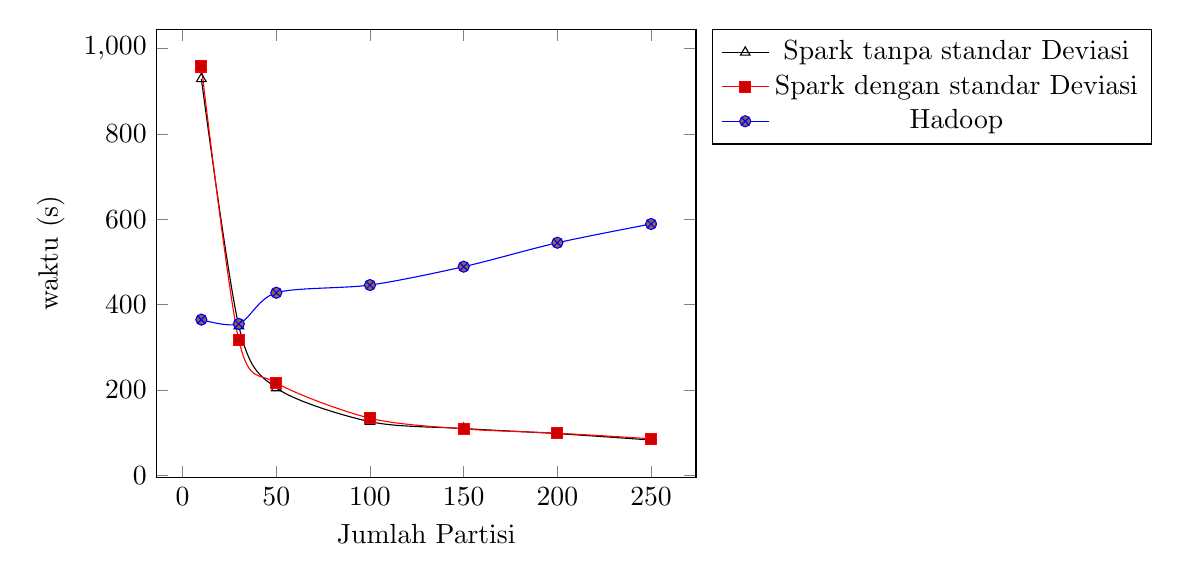
\begin{tikzpicture}[scale=\scl]
		\begin{axis}[\ymin,\ymax,xlabel= Jumlah Partisi,ylabel= waktu (s), xticklabel style={/pgf/number format/.cd, fixed,fixed zerofill, precision=0},legend pos = outer north east]
		
		\addlegendentry{Spark tanpa standar Deviasi}
		\addplot+[smooth][color=black,mark=triangle] coordinates {(10,929) (30,350) (50,205) (100,126) (150,110) (200,98) (250,83)};
		\addlegendentry{Spark dengan standar Deviasi}
		\addplot+[smooth][color=red] coordinates {
		(10,958) (30,317) (50,217) (100,134) (150,109) (200,99) (250,86)};
		\addlegendentry{Hadoop}
		\addplot+[smooth][color=blue] coordinates {(10,365) (30,355) (50,428) (100,446) (150,489) (200,545) (250,589)};

		

		\leg
		\end{axis}
		\end{tikzpicture}
		\caption[Hasil Percobaan Partisi Spark dan Hadoop dengan ukuran data 2GB, jumlah objek maksimum 30, dan total 10 core]{Hasil Percobaan Partisi Spark dan Hadoop dengan ukuran data 2GB, jumlah objek maksimum 30, dan total 10 core}
		\label{fig:percobaan2}
	\end{figure}
\end{minipage}\\



Berdasarkan hasil grafik pada Gambar~\ref{fig:percobaan2}, dapat dilihat bahwa waktu eksekusi Spark menurun dan waktu eksekusi Hadoop meningkat ketika jumlah partisi diperbesar. Waktu eksekusi Hadoop menaik secara konsisten ketika jumlah partisi diperbesar. Waktu eksekusi Spark menurun drastis pada awalnya ketika jumlah partisi ditingkatkan sampai titik tertentu dimana peningkatan jumlah partisi tidak memiliki dampak yang sangat drastis pada waktu eksekusi Spark. Tidak ada perbedaan yang jauh antara waktu eksekusi aplikasi Spark dengan standar deviasi maupun yang tidak. Aplikasi Spark memiliki waktu eksekusi yang lebih baik dibanding Hadoop pada jumlah partisi yang besar dan waktu eksekusi yang lebih buruk pada jumlah partisi yang kecil. Waktu eksekusi Spark pada partisi yang besar lebih cepat dibanding waktu eksekusi Hadoop terkecil. Aplikasi Spark lebih cepat dibanding Hadoop selama jumlah partisi diatur dengan benar.\\




%333333333333333333GBBBBBBBBBBBBBBBBB


Percobaan ini menguji waktu eksekusi Spark dan Hadoop berdasarkan jumlah partisi yang berbeda. Percobaan ini menggunakan 1 komputer sebagai komputer master dan 10 komputer lainya sebagai worker dengan setiap worker munggunakan 1 core. Ukuran data yang digunakan adalah 3 GB. Metode yang digunakan adalah metode \textit{single linkage} dengan nilai \textit{cut-off distance} adalah 0,8 dan jumlah objek maksimum untuk setiap \textit{dendrogram} adalah 30. Tabel~\ref{tab:spark3} berikut adalah hasil dari eksperimen:

\begin{table}[H] 
	\centering 
	\caption{Percobaan Jumlah Partisi Hadoop dan Spark dengan Ukuran Data 3 GB}
	\label{tab:spark3}
	\begin{tabular}{|p{1cm}|p{1cm}|p{2cm}|p{2cm}|p{2cm}|p{2cm}|p{2cm}|p{2cm}|}
\hline
Ukuran Data (GB) & Jumlah Partisi &  Waktu eksekusi Spark Tanpa standar Deviasi (Detik) & Waktu Eksekusi Spark (Detik) & Waktu Eksekusi Hadoop (Detik) & Hasil Reduksi Spark Tanpa standar Deviasi (GB) & Hasil Reduksi Spark (GB)  & Hasil Reduksi Hadoop (GB)\\ 
\hline
3 & 10 & 1446 & 1376 & 455 & 1.2 & 1.5 & 1.2 \\
\hline
3 & 30 & 516 & 491 & 445 & 1.2 & 1.5 & 1.2 \\
\hline
3 & 50 & 315 & 298 & 501 & 1.2 & 1.5 & 1.2 \\
\hline
3 & 100 & 188 & 183 & 532 & 1.2 & 1.5 & 1.2 \\
\hline
3 & 150 & 144 & 146 & 639 & 1.2 & 1.5 & 1.2 \\
\hline
3 & 200 & 135 & 144 & 720 & 1.2 & 1.5 & 1.2 \\
\hline
3 & 250 & 211 & 191 & 761 & 1.2 & 1.5 & 1.2 \\
\hline
3 & 300 & 182 & 176 & 822 & 1.2 & 1.5 & 1.2 \\
\hline
3 & 350 & 163 & 169 & 903 & 1.2 & 1.5 & 1.2 \\
\hline
3 & 400 & 137 & 158 & 1012 & 1.2 & 1.5 & 1.2 \\
\hline


\hline

	\end{tabular} 
\end{table}



\def\scl{1}

\def\leg{} 
\def\std{none}
\def\ymin{}
\def\ymax{}

\begin{minipage}[c]{0.9\textwidth}
	\begin{figure}[H]
		\centering
		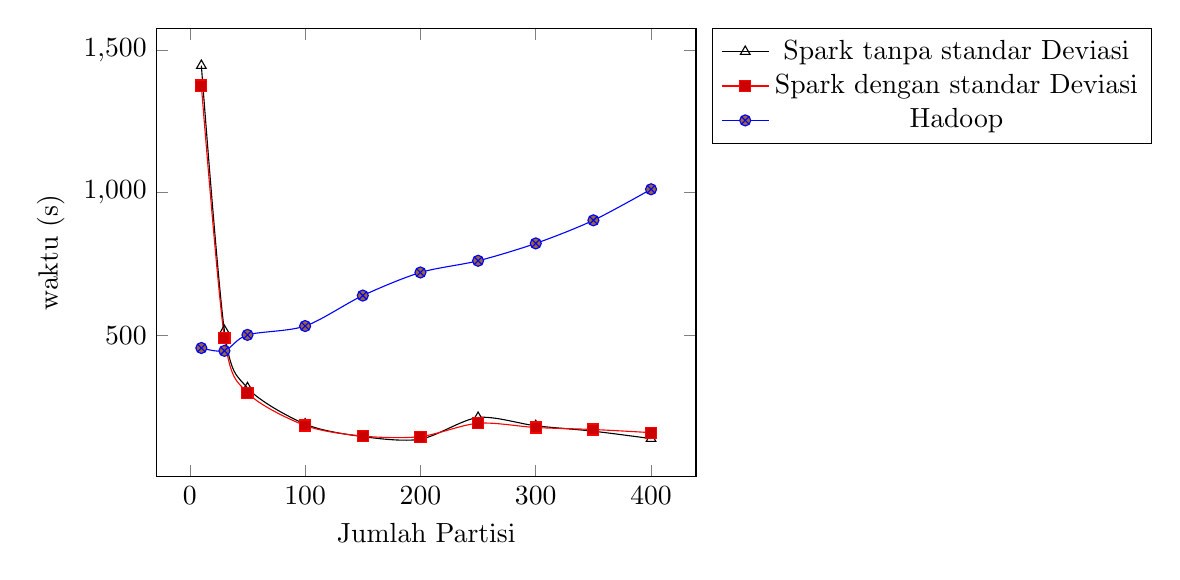
\begin{tikzpicture}[scale=\scl]
		\begin{axis}[\ymin,\ymax,xlabel= Jumlah Partisi,ylabel= waktu (s), xticklabel style={/pgf/number format/.cd, fixed,fixed zerofill, precision=0},legend pos = outer north east]
		
		\addlegendentry{Spark tanpa standar Deviasi}
		\addplot+[smooth][color=black,mark=triangle] coordinates {(10,1446) (30,516) (50,315) (100,188) (150,144) (200,135) (250,211) (300,182) (350,163) (400,137)};
		\addlegendentry{Spark dengan standar Deviasi}
		\addplot+[smooth][color=red] coordinates {
		(10,1376) (30,491) (50,298) (100,183) (150,146) (200,144) (250,191) (300,176) (350,169) (400,158)};
		\addlegendentry{Hadoop}
		\addplot+[smooth][color=blue] coordinates {(10,455) (30,445) (50,501) (100,532) (150,639) (200,720) (250,761) (300,822) (350,903) (400,1012)};

		

		\leg
		\end{axis}
		\end{tikzpicture}
		\caption[Hasil Percobaan Partisi Spark dan Hadoop dengan ukuran data 3GB, Objek Maksimum 30, dan Total 10 Core]{Hasil Percobaan Partisi Spark dan Hadoop dengan ukuran data 3GB, Objek Maksimum 30, dan Total 10 Core}
		\label{fig:percobaan3}
	\end{figure}
\end{minipage}\\



Berdasarkan hasil grafik pada Gambar~\ref{fig:percobaan3}, dapat dilihat bahwa waktu eksekusi Spark menurun dan waktu eksekusi Hadoop meningkat ketika jumlah partisi diperbesar. Waktu eksekusi Hadoop menaik secara konsisten ketika jumlah partisi diperbesar. Waktu eksekusi Spark menurun drastis pada awalnya ketika jumlah partisi ditingkatkan sampai titik tertentu dimana peningkatan jumlah partisi tidak memiliki dampak yang sangat drastis pada waktu eksekusi Spark. Tidak ada perbedaan yang jauh antara waktu eksekusi aplikasi Spark dengan standar deviasi maupun yang tidak. Aplikasi Spark memiliki waktu eksekusi yang lebih baik dibanding Hadoop pada jumlah partisi yang besar dan waktu eksekusi yang lebih buruk pada jumlah partisi yang kecil. Waktu eksekusi Spark pada partisi yang besar lebih cepat dibanding waktu eksekusi Hadoop terkecil. Aplikasi Spark lebih cepat dibanding Hadoop selama jumlah partisi diatur dengan benar.\\

%555555555555GBBBBBBBBBBBBBBBBB


Percobaan ini menguji waktu eksekusi Spark dan Hadoop berdasarkan jumlah partisi yang berbeda. Percobaan ini menggunakan 1 komputer sebagai komputer master dan 10 komputer lainya sebagai worker dengan setiap worker munggunakan 1 core. Ukuran data yang digunakan adalah 5 GB. Metode yang digunakan adalah metode \textit{single linkage} dengan nilai \textit{cut-off distance} adalah 0,8 dan jumlah objek maksimum untuk setiap \textit{dendrogram} adalah 30. Tabel~\ref{tab:spark5} berikut adalah hasil dari eksperimen:

\begin{table}[H] 
	\centering 
	\caption{Percobaan Jumlah Partisi Hadoop dan Spark dengan Ukuran Data 5 GB}
	\label{tab:spark5}
	\begin{tabular}{|p{1cm}|p{1cm}|p{2cm}|p{2cm}|p{2cm}|p{2cm}|p{2cm}|p{2cm}|}
\hline
Ukuran Data (GB) & Jumlah Partisi &  Waktu eksekusi Spark Tanpa standar Deviasi (Detik) & Waktu Eksekusi Spark (Detik) & Waktu Eksekusi Hadoop (Detik) & Hasil Reduksi Spark Tanpa standar Deviasi (GB) & Hasil Reduksi Spark (GB)  & Hasil Reduksi Hadoop (GB)\\ 
\hline
5  & 10 & 4490 & 4457 & 817 & 2.1 & 2.6 & 2.2\\
\hline
5  & 30 & 1637 & 2002 & 759 & 2.1 & 2.6 & 2.2\\
\hline
5  & 50 & 995 & 891 & 906 & 2.1 & 2.6 & 2.2 \\
\hline
5  & 100 & 524 & 590 & 952 & 2.1 & 2.6 & 2.2 \\
\hline
5  & 150 & 343 & 431 & 1121 & 2.1 & 2.6 & 2.2\\
\hline
5  & 200 & 315 & 288 & 1173 & 2.1 & 2.6 & 2.2\\
\hline
5  & 300 & 519 & 526 & 1485 & 2.1 & 2.6 & 2.2\\
\hline
5  & 400 & 422 & 399 & 2261 & 2.1 & 2.6 & 2.2 \\
\hline
5  & 500 & 359 & 370 & 1994 & 2.1 & 2.6 & 2.2\\
\hline
5  & 600 & 319 & 326 & 2282 & 2.1 & 2.6 & 2.2\\
\hline
5  & 700 & 259 & 306 & 2569 & 2.1 & 2.6 & 2.2\\
\hline
5  & 800 & 255 & 256 & 4463 & 2.1 & 2.6 & 2.2\\
\hline


\hline

	\end{tabular} 
\end{table}




\def\scl{1}

\def\leg{} 
\def\std{none}
\def\ymin{}
\def\ymax{}

\begin{minipage}[c]{0.9\textwidth}
	\begin{figure}[H]
		\centering
		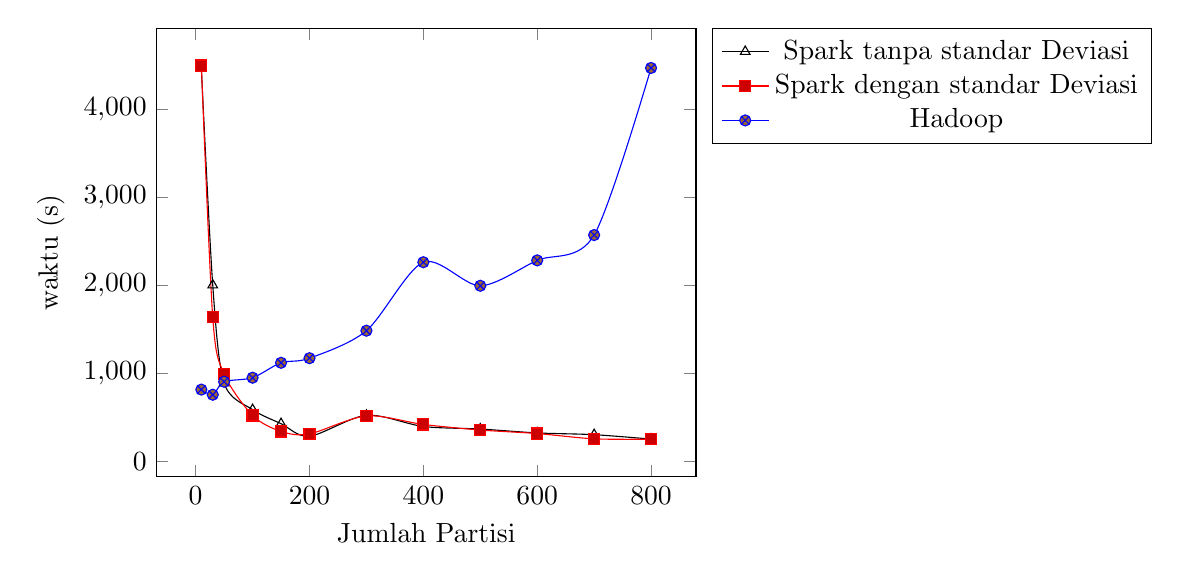
\begin{tikzpicture}[scale=\scl]
		\begin{axis}[\ymin,\ymax,xlabel= Jumlah Partisi,ylabel= waktu (s), xticklabel style={/pgf/number format/.cd, fixed,fixed zerofill, precision=0},legend pos = outer north east]
		
		\addlegendentry{Spark tanpa standar Deviasi}
		\addplot+[smooth][color=black,mark=triangle] coordinates {(10,4457) (30,2002) (50,891) (100,590) (150,431) (200,288) (300,526) (400,399) (500,370) (600,326) (700,306) (800,256)};
		\addlegendentry{Spark dengan standar Deviasi}
		\addplot+[smooth][color=red] coordinates {(10,4490) (30,1637) (50,995) (100,524) (150,343) (200,315) (300,519) (400,422) (500,359) (600,319) (700,259) (800,255)};
		\addlegendentry{Hadoop}
		\addplot+[smooth][color=blue] coordinates {(10,817) (30,759) (50,906) (100,952) (150,1121) (200,1173) (300,1485) (400,2261) (500,1994) (600,2282) (700,2569) (800,4463)};

		

		\leg
		\end{axis}
		\end{tikzpicture}
		\caption[Hasil Percobaan Partisi Spark dan Hadoop dengan ukuran data 5GB, Objek Maksimum 30, dan Total 10 Core]{Hasil Percobaan Partisi Spark dan Hadoop dengan ukuran data 5GB, Objek Maksimum 30, dan Total 10 Core}
		\label{fig:percobaan4}
	\end{figure}
\end{minipage}\\

Berdasarkan hasil grafik pada Gambar~\ref{fig:percobaan4}, dapat dilihat bahwa waktu eksekusi Spark menurun dan waktu eksekusi Hadoop meningkat ketika jumlah partisi diperbesar. Waktu eksekusi Hadoop menaik secara konsisten ketika jumlah partisi diperbesar. Waktu eksekusi Spark menurun drastis pada awalnya ketika jumlah partisi ditingkatkan sampai titik tertentu dimana peningkatan jumlah partisi tidak memiliki dampak yang sangat drastis pada waktu eksekusi Spark. Tidak ada perbedaan yang jauh antara waktu eksekusi aplikasi Spark dengan standar deviasi maupun yang tidak. Aplikasi Spark memiliki waktu eksekusi yang lebih baik dibanding Hadoop pada jumlah partisi yang besar dan waktu eksekusi yang lebih buruk pada jumlah partisi yang kecil. Waktu eksekusi Spark pada partisi yang besar lebih cepat dibanding waktu eksekusi Hadoop terkecil. Aplikasi Spark lebih cepat dibanding Hadoop selama jumlah partisi diatur dengan benar.\\



%100000000000000000GBBBBBBBBBBBBBBBBB



Percobaan ini menguji waktu eksekusi Spark dan Hadoop berdasarkan jumlah partisi yang berbeda. Percobaan ini menggunakan 1 komputer sebagai komputer master dan 10 komputer lainya sebagai worker dengan setiap worker munggunakan 1 core. Ukuran data yang digunakan adalah 10 GB. Metode yang digunakan adalah metode \textit{single linkage} dengan nilai \textit{cut-off distance} adalah 0,8 dan jumlah objek maksimum untuk setiap \textit{dendrogram} adalah 30. Tabel~\ref{tab:spark6} dan Tabel~\ref{tab:spark7} berikut adalah hasil dari eksperimen:

\begin{table}[H] 
	\centering 
	\caption{Percobaan Jumlah Partisi Spark dengan Ukuran Data 10 GB}
	\label{tab:spark6}
	\begin{tabular}{|p{1cm}|p{1cm}|p{3cm}|p{3cm}|p{3cm}|p{3cm}|}
\hline
Ukuran Data (GB) & Jumlah Partisi &  Waktu eksekusi Spark Tanpa standar Deviasi (Detik) & Waktu Eksekusi Spark (Detik) & Hasil Reduksi Spark Tanpa standar Deviasi (GB) & Hasil Reduksi Spark (GB)  \\ 
\hline
10 & 50 & 7254 & 7236 & 3.7 & 4.6 \\
\hline
10 & 100 & 237 & 2805 &  3.7 & 4.6 \\
\hline
10 & 200 & 1736 & 1718 & 3.7 & 4.6 \\
\hline
10 & 300 & 1477 & 1494 & 3.7 & 4.6 \\
\hline
10 & 400 & 1160 & 1207 & 3.7 & 4.6 \\
\hline
10 & 500 & 923 & 984 &  3.7 & 4.6 \\
\hline
10 & 600 & 774 & 780 & 3.7 & 4.6 \\
\hline
10 & 700 & 645 & 652 & 3.7 & 4.6 \\
\hline
10 & 900 & 563 & 568 & 3.7 & 4.6 \\
\hline
10 & 1100 & 522 & 524 & 3.7 & 4.6 \\
\hline
10 & 1300 & 359 & 504 & 3.7 & 4.6 \\
\hline
10 & 1500 & 255 & 256 & 3.7 & 4.6 \\
\hline


\hline

	\end{tabular} 
\end{table}



\begin{table}[H] 
	\centering 
	\caption{Percobaan Jumlah Partisi Hadoop dengan Ukuran Data 10 GB}
	\label{tab:spark7}
	\begin{tabular}{|p{3cm}|p{2.5cm}|p{4cm}|p{3.5cm}|}
\hline
Ukuran Data (GB) & Jumlah Partisi &  Waktu Eksekusi Hadoop (Detik) & Hasil Reduksi Hadoop (GB)\\
\hline
10 & 10 & 1260 & 3.9 \\
\hline
10 & 30 & 1446 & 3.9 \\
\hline
10 & 50 & 1481 & 3.9 \\
\hline
10 & 100 & 1631 & 3.9 \\
\hline
10 & 200 & 2127 & 3.9 \\
\hline
10 & 300 & 2583 & 3.9 \\
\hline
10 & 400 & 3721 & 3.9 \\
\hline
10 & 500 & 3573 & 3.9 \\
\hline
10 & 700 & 5014 & 3.9 \\
\hline
10 & 900 & 5529 & 3.9 \\
\hline
10 & 1100 & 7254 & 3.9 \\
\hline
10 & 1300 & 8989 & 3.9 \\
\hline
10 & 1500 & 9499 & 3.9 \\
\hline


\hline

	\end{tabular} 
\end{table}



\def\scl{1}

\def\leg{} 
\def\std{none}
\def\ymin{}
\def\ymax{}

\begin{minipage}[c]{0.9\textwidth}
	\begin{figure}[H]
		\centering
		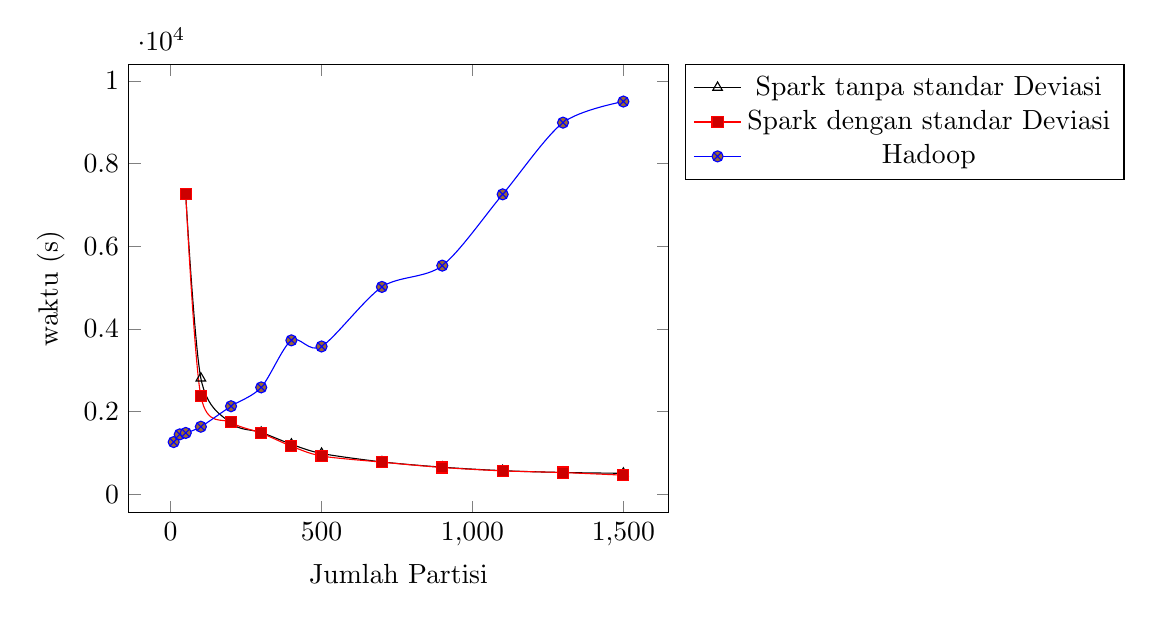
\begin{tikzpicture}[scale=\scl]
		\begin{axis}[\ymin,\ymax,xlabel= Jumlah Partisi,ylabel= waktu (s), xticklabel style={/pgf/number format/.cd, fixed,fixed zerofill, precision=0},legend pos = outer north east]
		
		\addlegendentry{Spark tanpa standar Deviasi}
		\addplot+[smooth][color=black,mark=triangle] coordinates {(50,7236) (100,2805) (200,1718) (300,1494) (400,1207) (500,984) (700,780) (900,652) (1100,568) (1300,524) (1500,504)};
		\addlegendentry{Spark dengan standar Deviasi}
		\addplot+[smooth][color=red] coordinates {(50,7254) (100,2373) (200,1736) (300,1477) (400,1160) (500,923) (700,774) (900,645) (1100,563) (1300,522) (1500,459)};
		\addlegendentry{Hadoop}
		\addplot+[smooth][color=blue] coordinates {(10,1260) (30,1446) (50,1481) (100,1631) (200,2127) (300,2583) (400,3721) (500,3573) (700,5014) (900,5529) (1100,7254) (1300,8989) (1500,9499)};

		

		\leg
		\end{axis}
		\end{tikzpicture}
		\caption[Hasil Percobaan Partisi Spark dan Hadoop dengan ukuran data 10GB, Objek Maksimum 30, dan Total 10 Core]{Hasil Percobaan Partisi Spark dan Hadoop dengan ukuran data 10GB, Objek Maksimum 30, dan Total 10 Core}
		\label{fig:percobaan5}
	\end{figure}
\end{minipage}\\

Berdasarkan hasil grafik pada Gambar~\ref{fig:percobaan5}, dapat dilihat bahwa waktu eksekusi Spark menurun dan waktu eksekusi Hadoop meningkat ketika jumlah partisi diperbesar. Waktu eksekusi Hadoop menaik secara konsisten ketika jumlah partisi diperbesar. Waktu eksekusi Spark menurun drastis pada awalnya ketika jumlah partisi ditingkatkan sampai titik tertentu dimana peningkatan jumlah partisi tidak memiliki dampak yang sangat drastis pada waktu eksekusi Spark. Tidak ada perbedaan yang jauh antara waktu eksekusi aplikasi Spark dengan standar deviasi maupun yang tidak. Aplikasi Spark memiliki waktu eksekusi yang lebih baik dibanding Hadoop pada jumlah partisi yang besar dan waktu eksekusi yang lebih buruk pada jumlah partisi yang kecil. Waktu eksekusi Spark pada partisi yang besar lebih cepat dibanding waktu eksekusi Hadoop terkecil. Aplikasi Spark lebih cepat dibanding Hadoop selama jumlah partisi diatur dengan benar.\\




%1111111111555555555555GBBBBBBBBBBBBBBBBB


Percobaan ini menguji waktu eksekusi Spark dan Hadoop berdasarkan jumlah partisi yang berbeda. Percobaan ini menggunakan 1 komputer sebagai komputer master dan 10 komputer lainya sebagai worker dengan setiap worker munggunakan 1 core. Ukuran data yang digunakan adalah 15 GB. Metode yang digunakan adalah metode \textit{single linkage} dengan nilai \textit{cut-off distance} adalah 0,8 dan jumlah objek maksimum untuk setiap \textit{dendrogram} adalah 30. Tabel~\ref{tab:spark7} dan Tabel~\ref{tab:spark8} berikut adalah hasil dari eksperimen:

\begin{table}[H] 
	\centering 
	\caption{Percobaan Jumlah Partisi Spark dengan Ukuran Data 15 GB}
	\label{tab:spark7}
	\begin{tabular}{|p{1cm}|p{1cm}|p{3cm}|p{3cm}|p{3cm}|p{3cm}|}
\hline
Ukuran Data ) & Jumlah Partisi &  Waktu eksekusi Spark Tanpa standar Deviasi (GB) & Waktu Eksekusi Spark (detik) & Hasil Reduksi Spark Tanpa standar Deviasi ) & Hasil Reduksi Spark )  \\ 
\hline
15 & 100 & 9034  & 9294  &  5.8 & 7.3 \\
\hline
15 & 200 & 5239  & 4847  & 5.8 & 7.3 \\
\hline
15 & 300 & 3263  & 3761  & 5.8 & 7.3 \\
\hline
15 & 500 & 2175  & 2024  &  5.8 & 7.3 \\
\hline
15 & 700 & 1645  & 1696  & 5.8 & 7.3 \\
\hline
15 & 900 & 1276  & 1372  & 5.8 & 7.3 \\
\hline
15 & 1200 & 1136  & 1114  & 5.8 & 7.3 \\
\hline
15 & 1500 & 970  & 918  & 5.8 & 7.3 \\
\hline
15 & 1800 & 834  & 863  & 5.8 & 7.3 \\
\hline
15 & 2100 & 773  & 783  & 5.8 & 7.3 \\
\hline
15 & 2400 & 739  & 738  & 5.8 & 7.3 \\
\hline

\hline

	\end{tabular} 
\end{table}



\begin{table}[H] 
	\centering 
	\caption{Percobaan Jumlah Partisi Hadoop dengan Ukuran Data 15 GB}
	\label{tab:spark8}
	\begin{tabular}{|p{3cm}|p{3cm}|p{4cm}|p{4cm}|}
\hline
Ukuran Data (GB) & Jumlah Partisi &  Waktu Eksekusi Hadoop (detik) & Hasil Reduksi Hadoop (GB)\\
\hline
15 & 10 & 2133  & 3.9 \\
\hline
15 & 30 & 2177  & 3.9 \\
\hline
15 & 50 & 2234  & 3.9 \\
\hline
15 & 100 & 2474  & 3.9 \\
\hline
15 & 200 & 3306  & 3.9 \\
\hline
15 & 300 & 4655  & 3.9 \\
\hline
15 & 400 & 4775  & 3.9 \\
\hline
15 & 500 & 6644  & 3.9 \\
\hline
15 & 700 & 8203  & 3.9 \\
\hline
15 & 900 & 8482  & 3.9 \\
\hline


\hline

	\end{tabular} 
\end{table}


\def\scl{1}

\def\leg{} 
\def\std{none}
\def\ymin{}
\def\ymax{}

\begin{minipage}[c]{0.9\textwidth}
	\begin{figure}[H]
		\centering
		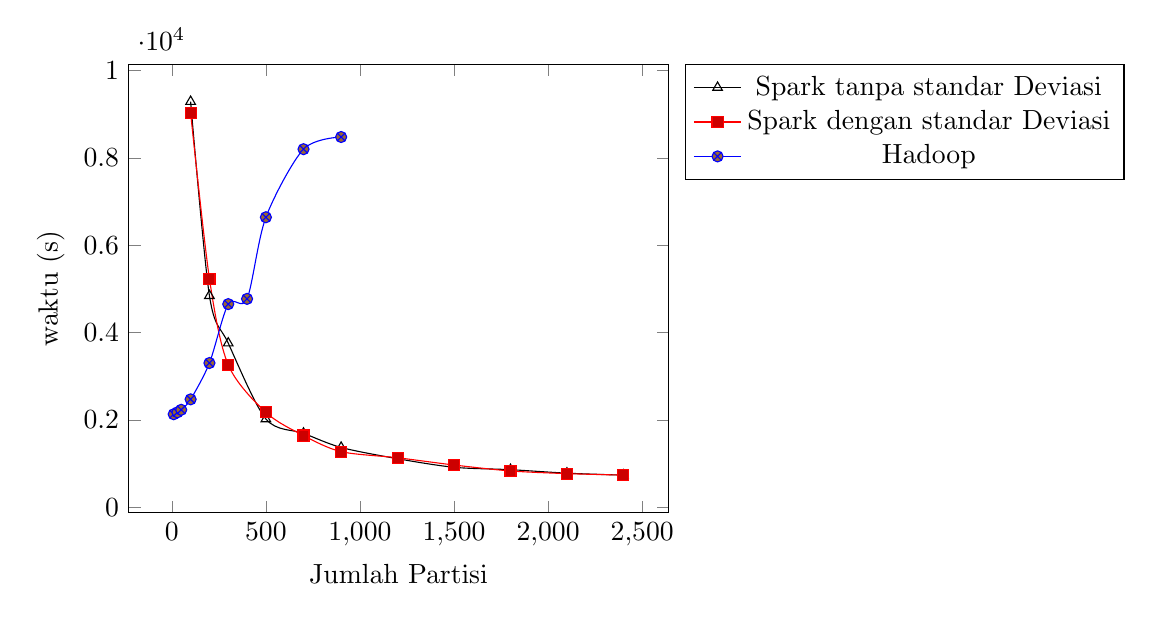
\begin{tikzpicture}[scale=\scl]
		\begin{axis}[\ymin,\ymax,xlabel= Jumlah Partisi,ylabel= waktu (s), xticklabel style={/pgf/number format/.cd, fixed,fixed zerofill, precision=0},legend pos = outer north east]
		
		\addlegendentry{Spark tanpa standar Deviasi}
		\addplot+[smooth][color=black,mark=triangle] coordinates { (100,9294) (200,4847) (300,3761) (500,2024) (700,1696) (900,1372) (1200,1114) (1500,918) (1800,863) (2100,783) (2400,738)};
		\addlegendentry{Spark dengan standar Deviasi}
		\addplot+[smooth][color=red] coordinates {(100,9034) (200,5239) (300,3263) (500,2175) (700,1645) (900,1276) (1200,1136) (1500,970) (1800,834) (2100,773) (2400,739)};
		\addlegendentry{Hadoop}
		\addplot+[smooth][color=blue] coordinates {(10,2133) (30,2177) (50,2234) (100,2474) (200,3306) (300,4655) (400,4775) (500,6644) (700,8203) (900,8482)};

		

		\leg
		\end{axis}
		\end{tikzpicture}
		\caption[Hasil Percobaan Partisi Spark dan Hadoop dengan ukuran data 15GB, Objek Maksimum 30, dan Total 10 Core]{Hasil Percobaan Partisi Spark dan Hadoop dengan ukuran data 15GB, Objek Maksimum 30, dan Total 10 Core}
		\label{fig:percobaan6}
	\end{figure}
\end{minipage}\\

Berdasarkan hasil grafik pada Gambar~\ref{fig:percobaan6}, dapat dilihat bahwa waktu eksekusi Spark menurun dan waktu eksekusi Hadoop meningkat ketika jumlah partisi diperbesar. Waktu eksekusi Hadoop menaik secara konsisten ketika jumlah partisi diperbesar. Waktu eksekusi Spark menurun drastis pada awalnya ketika jumlah partisi ditingkatkan sampai titik tertentu dimana peningkatan jumlah partisi tidak memiliki dampak yang sangat drastis pada waktu eksekusi Spark. Tidak ada perbedaan yang jauh antara waktu eksekusi aplikasi Spark dengan standar deviasi maupun yang tidak. Aplikasi Spark memiliki waktu eksekusi yang lebih baik dibanding Hadoop pada jumlah partisi yang besar dan waktu eksekusi yang lebih buruk pada jumlah partisi yang kecil. Waktu eksekusi Spark pada partisi yang besar lebih cepat dibanding waktu eksekusi Hadoop terkecil. Aplikasi Spark lebih cepat dibanding Hadoop selama jumlah partisi diatur dengan benar.\\


%2222222222222200000000000000000GBBBBBBBBBBBBBBBBB


Percobaan ini menguji waktu eksekusi Spark dan Hadoop berdasarkan jumlah partisi yang berbeda. Percobaan ini menggunakan 1 komputer sebagai komputer master dan 10 komputer lainya sebagai worker dengan setiap worker munggunakan 1 core. Ukuran data yang digunakan adalah 20 GB. Metode yang digunakan adalah metode \textit{single linkage} dengan nilai \textit{cut-off distance} adalah 0,8 dan jumlah objek maksimum untuk setiap \textit{dendrogram} adalah 30. Tabel~\ref{tab:spark9} dan Tabel~\ref{tab:spark10} berikut adalah hasil dari eksperimen:

\begin{table}[H] 
	\centering 
	\caption{Percobaan Jumlah Partisi Spark dengan Ukuran Data 20 GB}
	\label{tab:spark9}
	\begin{tabular}{|p{1cm}|p{1cm}|p{3cm}|p{3cm}|p{3cm}|p{3cm}|}
\hline
Ukuran Data (GB) & Jumlah Partisi &  Waktu eksekusi Spark Tanpa standar Deviasi (detik) & Waktu Eksekusi Spark (detik) & Hasil Reduksi Spark Tanpa standar Deviasi (GB) & Hasil Reduksi Spark (GB)  \\ 
\hline
20 & 200 & 8866  & 8386  & 7.7 & 9.6 \\
\hline
20 & 400 & 4553  & 4342  & 7.7 & 9.6 \\
\hline
20 & 600 & 3021  & 2841  &  7.7 & 9.6 \\
\hline
20 & 1000 & 2084  & 2065  & 7.7 & 9.6 \\
\hline
20 & 1400 & 1471  & 1598  & 7.7 & 9.6 \\
\hline
20 & 1800 & 1298  & 1372  & 7.7 & 9.6 \\
\hline
20 & 2200 & 1165  & 1228  & 7.7 & 9.6 \\
\hline
20 & 2600 & 1081  & 1133  & 7.7 & 9.6 \\
\hline
20 & 3000 & 1031  & 1010  & 7.7 & 9.6 \\
\hline

\hline

	\end{tabular} 
\end{table}



\begin{table}[H] 
	\centering 
	\caption{Percobaan Jumlah Partisi Hadoop dengan Ukuran Data 20 GB}
	\label{tab:spark10}
	\begin{tabular}{|p{3cm}|p{3cm}|p{4cm}|p{4cm}|}
\hline
Ukuran Data (GB) & Jumlah Partisi &  Waktu Eksekusi Hadoop (detik) & Hasil Reduksi Hadoop (GB)\\
\hline
20 & 10 & 2763  & 8.1 \\
\hline
20 & 30 & 2811  & 8.1 \\
\hline
20 & 50 & 3007  & 8.1  \\
\hline
20 & 100 & 3261  & 8.1 \\
\hline
20 & 200 & 4360  & 8.1 \\
\hline
20 & 400 & 6249  & 8.1 \\
\hline
20 & 700 & 10476  & 8.1 \\
\hline
20 & 1000 & 13839  & 8.1 \\
\hline


\hline

	\end{tabular} 
\end{table}



\def\scl{1}

\def\leg{} 
\def\std{none}
\def\ymin{}
\def\ymax{}

\begin{minipage}[c]{0.9\textwidth}
	\begin{figure}[H]
		\centering
		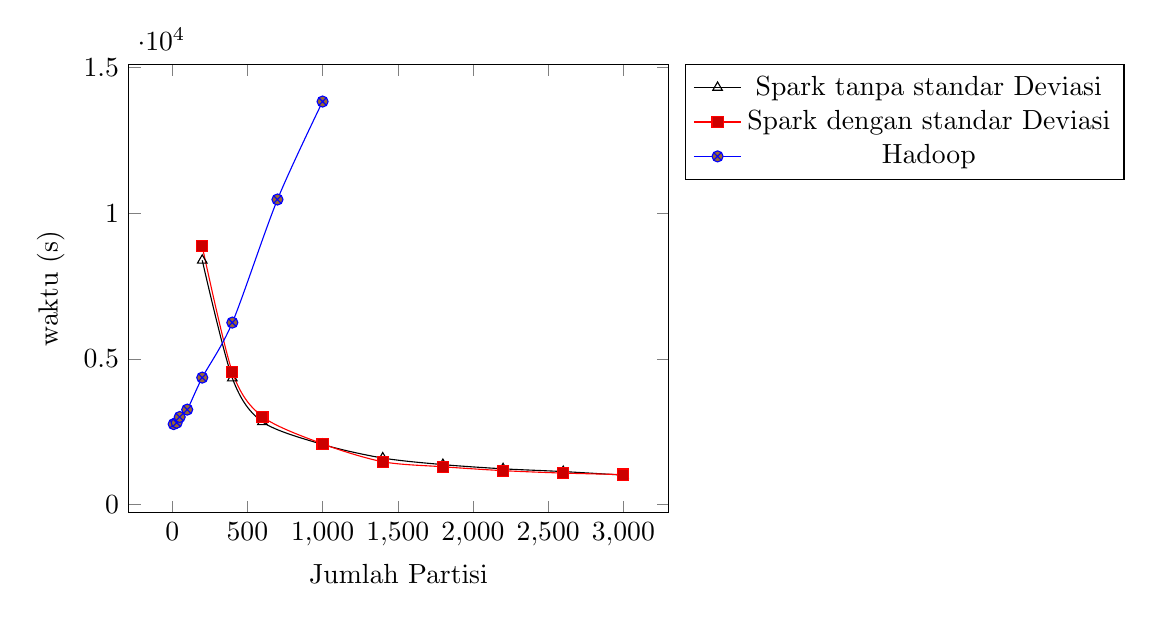
\begin{tikzpicture}[scale=\scl]
		\begin{axis}[\ymin,\ymax,xlabel= Jumlah Partisi,ylabel= waktu (s), xticklabel style={/pgf/number format/.cd, fixed,fixed zerofill, precision=0},legend pos = outer north east]
		
		\addlegendentry{Spark tanpa standar Deviasi}
		\addplot+[smooth][color=black,mark=triangle] coordinates { (200,8386) (400,4342) (600,2841) (1000,2065) (1400,1598) (1800,1372) (2200,1228) (2600,1133) (3000,1010)};
		\addlegendentry{Spark dengan standar Deviasi}
		\addplot+[smooth][color=red] coordinates {(200,8866) (400,4553) (600,3021) (1000,2084) (1400,1471) (1800,1298) (2200,1165) (2600,1081) (3000,1031)};
		\addlegendentry{Hadoop}
		\addplot+[smooth][color=blue] coordinates {(10,2763) (30,2811) (50,3007) (100,3261) (200,4360) (400,6249) (700,10476) (1000,13839)};

		

		\leg
		\end{axis}
		\end{tikzpicture}
		\caption[Hasil Percobaan Partisi Spark dan Hadoop dengan ukuran data 20GB, Objek Maksimum 30, dan Total 10 Core]{Hasil Percobaan Partisi Spark dan Hadoop dengan ukuran data 20GB, Objek Maksimum 30, dan Total 10 Core}
		\label{fig:percobaan7}
	\end{figure}
\end{minipage}\\


Berdasarkan hasil grafik pada Gambar~\ref{fig:percobaan7}, dapat dilihat bahwa waktu eksekusi Spark menurun dan waktu eksekusi Hadoop meningkat ketika jumlah partisi diperbesar. Waktu eksekusi Hadoop menaik secara konsisten ketika jumlah partisi diperbesar. Waktu eksekusi Spark menurun drastis pada awalnya ketika jumlah partisi ditingkatkan sampai titik tertentu dimana peningkatan jumlah partisi tidak memiliki dampak yang sangat drastis pada waktu eksekusi Spark. Tidak ada perbedaan yang jauh antara waktu eksekusi aplikasi Spark dengan standar deviasi maupun yang tidak. Aplikasi Spark memiliki waktu eksekusi yang lebih baik dibanding Hadoop pada jumlah partisi yang besar dan waktu eksekusi yang lebih buruk pada jumlah partisi yang kecil. Waktu eksekusi Spark pada partisi yang besar lebih cepat dibanding waktu eksekusi Hadoop terkecil. Aplikasi Spark lebih cepat dibanding Hadoop selama jumlah partisi diatur dengan benar.\\



%%%%%%%%%%%%%%%%MAX OBJ 50



%%%%%%%%%%%%%%%%%%%%%%%%%%%%%%%%%%%MAX OBJ 50 5 GB

Percobaan ini menguji waktu eksekusi Spark dan Hadoop berdasarkan jumlah partisi yang optimal. Percobaan ini menggunakan 1 komputer sebagai komputer \textit{master} dan 10 komputer lainya sebagai \textit{worker} dengan setiap \textit{worker} munggunakan 1 core. Ukuran data yang digunakan adalah 5 GB. Metode yang digunakan adalah metode \textit{single linkage} dengan nilai \textit{cut-off distance} adalah 0,8 dan jumlah objek maksimum untuk setiap \textit{dendrogram} adalah 50. Tabel~\ref{tab:spark11} dan Tabel~\ref{tab:spark12} berikut adalah hasil dari eksperimen:





\begin{table}[H] 
	\centering 
	\caption{Percobaan Jumlah Partisi Hadoop dengan Ukuran Data 5 GB}
	\label{tab:spark11}
	\begin{tabular}{|p{3cm}|p{3cm}|p{4cm}|p{4cm}|}
\hline
Ukuran Data (GB) & Jumlah Partisi &  Waktu Eksekusi Hadoop (detik) & Hasil Reduksi Hadoop (GB)\\
\hline
5 & 10 & 1546  & 1.5  \\
\hline
5 & 30 & 1571  & 1.5  \\
\hline
5 & 50 & 1654  & 1.5   \\
\hline
5 & 100 & 1721 & 1.5   \\
\hline
5 & 200 & 2076  & 1.5   \\
\hline


\hline

	\end{tabular} 
\end{table}






\begin{table}[H] 
	\centering 
	\caption{Percobaan Jumlah Partisi Spark dengan Ukuran Data 5 GB}
	\label{tab:spark12}
	\begin{tabular}{|p{1cm}|p{1cm}|p{3cm}|p{3cm}|p{3cm}|p{3cm}|}
\hline
Ukuran Data (GB) & Jumlah Partisi &  Waktu eksekusi Spark Tanpa standar Deviasi (detik) & Waktu Eksekusi Spark (detik) & Hasil Reduksi Spark Tanpa standar Deviasi (GB) & Hasil Reduksi Spark (GB)  \\ 
\hline
5 & 300 & 394 &  433  & 1.5  & 1.9 \\
\hline
5 & 400 & 368  & 381  & 1.5  & 1.9 \\
\hline
5 & 500 & 342  & 364  & 1.5  & 1.9 \\
\hline
5 & 600 & 331  & 353  &  1.5  & 1.9 \\
\hline
5 & 700 &  323 &  320  &  1.5  & 1.9 \\
\hline

\hline

	\end{tabular} 
\end{table}



\def\scl{1}

\def\leg{} 
\def\std{none}
\def\ymin{}
\def\ymax{}

\begin{minipage}[c]{0.9\textwidth}
	\begin{figure}[H]
		\centering
		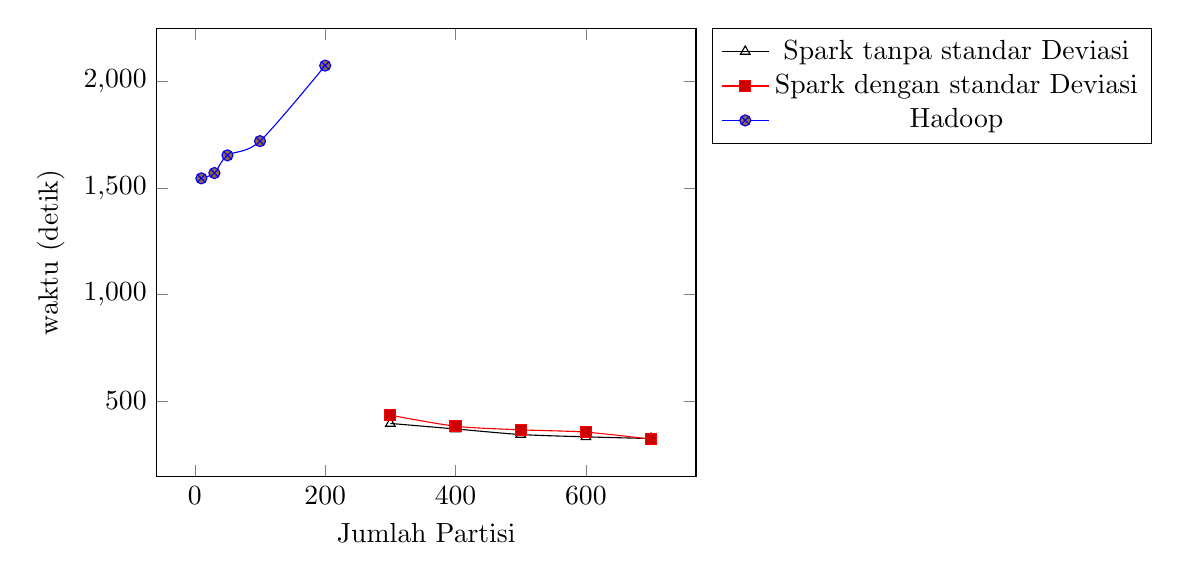
\begin{tikzpicture}[scale=\scl]
		\begin{axis}[\ymin,\ymax,xlabel= Jumlah Partisi,ylabel= waktu (detik), xticklabel style={/pgf/number format/.cd, fixed,fixed zerofill, precision=0},legend pos = outer north east]
		
		\addlegendentry{Spark tanpa standar Deviasi}
		\addplot+[smooth][color=black,mark=triangle] coordinates { (300,394) (400,368) (500,342) (600,331) (700,323)};
		\addlegendentry{Spark dengan standar Deviasi}
		\addplot+[smooth][color=red] coordinates { (300,433) (400,381) (500,364) (600,353) (700,320)};
		\addlegendentry{Hadoop}
		\addplot+[smooth][color=blue] coordinates {(10,1546) (30,1571) (50,1654) (100,1721) (200,2076) };

		

		\leg
		\end{axis}
		\end{tikzpicture}
		\caption[Hasil Percobaan Jumlah Partisi Spark dan Hadoop dengan ukuran data 5GB, Objek Maksimum 50, dan Total 10 Core]{Hasil Percobaan Jumlah Partisi Spark dan Hadoop dengan Ukuran Data 5 GB, Objek Maksimum 50, dan Total 10 Core}
		\label{fig:percobaan9}
	\end{figure}
\end{minipage}\\



Berdasarkan hasil grafik pada Gambar~\ref{fig:percobaan9}, dapat dilihat waktu Hadoop terus meningkat seiring meningkatnya jumlah partisi. Jumlah partisi yang dicoba pada Hadoop hanya mencapai 200 karena waktu eksekusi yang sudah berbeda jauh dibanding Spark dan untuk partisi yang lebih besar pasti diatas waktu eksekusi Hadoop dengan jumlah partisi sama dengan 200. Spark memiliki waktu eksekusi yang jauh lebih cepat dibanding Hadoop.\\  

%%%%%%%%%%%%%%%%%%%%%%%%%%%%%%%%%%%MAX OBJ 50 10 GB


Percobaan ini menguji waktu eksekusi Spark dan Hadoop berdasarkan jumlah partisi yang optimal. Percobaan ini menggunakan 1 komputer sebagai komputer \textit{master} dan 10 komputer lainya sebagai \textit{worker} dengan setiap \textit{worker} munggunakan 1 core. Ukuran data yang digunakan adalah 10 GB. Metode yang digunakan adalah metode \textit{single linkage} dengan nilai \textit{cut-off distance} adalah 0,8 dan jumlah objek maksimum untuk setiap \textit{dendrogram} adalah 50. Tabel~\ref{tab:spark13} dan Tabel~\ref{tab:spark14} berikut adalah hasil dari eksperimen:





\begin{table}[H] 
	\centering 
	\caption{Percobaan Jumlah Partisi Hadoop dengan Ukuran Data 10 GB}
	\label{tab:spark13}
	\begin{tabular}{|p{3cm}|p{3cm}|p{4cm}|p{4cm}|}
\hline
Ukuran Data (GB) & Jumlah Partisi &  Waktu Eksekusi Hadoop (detik) & Hasil Reduksi Hadoop (GB)\\
\hline
10 & 10 & 2740  & 2.7  \\
\hline
10 & 30 & 2821  & 2.7  \\
\hline
10 & 50 & 2897 & 2.7   \\
\hline
10 & 100 & 3130 & 2.7   \\
\hline
10 & 200 & 3571 & 2.7   \\
\hline


\hline

	\end{tabular} 
\end{table}




\begin{table}[H] 
	\centering 
	\caption{Percobaan Jumlah Partisi Spark dengan Ukuran Data 10 GB}
	\label{tab:spark14}
	\begin{tabular}{|p{1cm}|p{1cm}|p{3cm}|p{3cm}|p{3cm}|p{3cm}|}
\hline
Ukuran Data (GB) & Jumlah Partisi &  Waktu eksekusi Spark Tanpa standar Deviasi (detik) & Waktu Eksekusi Spark (detik) & Hasil Reduksi Spark Tanpa standar Deviasi (GB) & Hasil Reduksi Spark (GB)  \\ 
\hline
10 & 500 &  740 &  741 & 2.7  & 3.3 \\
\hline
10 & 700 & 653  & 664  & 2.7  & 3.3 \\
\hline
10 & 900 & 582  & 565  & 2.7  & 3.3 \\
\hline
10 & 1100 & 625  & 540  &  2.7  & 3.3 \\
\hline
10 & 1300 &  557 &  561 &  2.7  & 3.3 \\
\hline

\hline

	\end{tabular} 
\end{table}



\def\scl{1}

\def\leg{} 
\def\std{none}
\def\ymin{}
\def\ymax{}

\begin{minipage}[c]{0.9\textwidth}
	\begin{figure}[H]
		\centering
		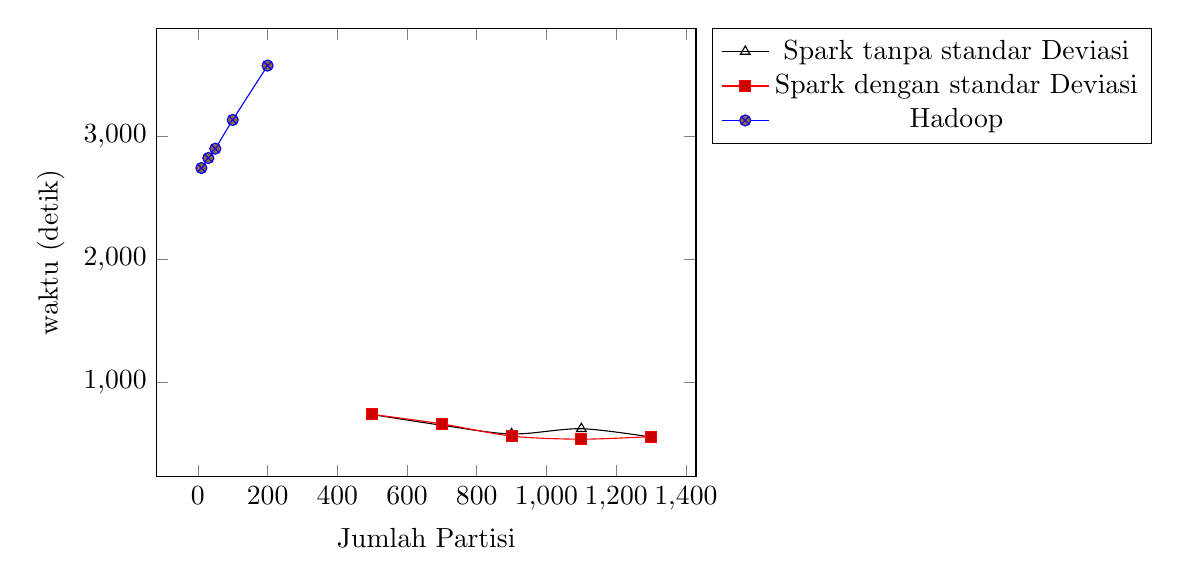
\begin{tikzpicture}[scale=\scl]
		\begin{axis}[\ymin,\ymax,xlabel= Jumlah Partisi,ylabel= waktu (detik), xticklabel style={/pgf/number format/.cd, fixed,fixed zerofill, precision=0},legend pos = outer north east]
		
		\addlegendentry{Spark tanpa standar Deviasi}
		\addplot+[smooth][color=black,mark=triangle] coordinates { (500,740) (700,653) (900,582) (1100,625) (1300,557)};
		\addlegendentry{Spark dengan standar Deviasi}
		\addplot+[smooth][color=red] coordinates { (500,741) (700,664) (900,565) (1100,540) (1300,561)};
		\addlegendentry{Hadoop}
		\addplot+[smooth][color=blue] coordinates {(10,2740) (30,2821) (50,2897) (100,3130) (200,3571) };

		

		\leg
		\end{axis}
		\end{tikzpicture}
		\caption[Hasil Percobaan Jumlah Partisi Spark dan Hadoop dengan Ukuran Data 10 GB, Objek Maksimum 50, dan Total 10 Core]{Hasil Percobaan Jumlah Partisi Spark dan Hadoop dengan Ukuran Data 10 GB, Objek Maksimum 50, dan Total 10 Core}
		\label{fig:percobaan10}
	\end{figure}
\end{minipage}\\



Berdasarkan hasil grafik pada Gambar~\ref{fig:percobaan10}, dapat dilihat waktu Hadoop terus meningkat seiring meningkatnya jumlah partisi. Jumlah partisi yang dicoba pada Hadoop hanya mencapai 200 karena waktu eksekusi yang sudah berbeda jauh dibanding Spark dan untuk partisi yang lebih besar pasti diatas waktu eksekusi Hadoop dengan jumlah partisi sama dengan 200. Spark memiliki waktu eksekusi yang jauh lebih cepat dibanding Hadoop.\\



%%%%%%%%%%%%%%%%%%%%%%%%%%%%%%%%%%%MAX OBJ 50 15 GB


Percobaan ini menguji waktu eksekusi Spark dan Hadoop berdasarkan jumlah partisi yang optimal. Percobaan ini menggunakan 1 komputer sebagai komputer \textit{master} dan 10 komputer lainya sebagai \textit{worker} dengan setiap \textit{worker} munggunakan 1 core. Ukuran data yang digunakan adalah 15 GB. Metode yang digunakan adalah metode \textit{single linkage} dengan nilai \textit{cut-off distance} adalah 0,8 dan jumlah objek maksimum untuk setiap \textit{dendrogram} adalah 50. Tabel~\ref{tab:spark15} dan Tabel~\ref{tab:spark16} berikut adalah hasil dari eksperimen:





\begin{table}[H] 
	\centering 
	\caption{Percobaan Jumlah Partisi Hadoop dengan Ukuran Data 15 GB}
	\label{tab:spark15}
	\begin{tabular}{|p{3cm}|p{3cm}|p{4cm}|p{4cm}|}
\hline
Ukuran Data (GB) & Jumlah Partisi &  Waktu Eksekusi Hadoop (detik) & Hasil Reduksi Hadoop (GB)\\
\hline
15 & 10 & 4273  & 4.2  \\
\hline
15 & 30 & 4319  & 4.2  \\
\hline
15 & 50 & 4479  & 4.2  \\
\hline
15 & 100 & 4674  & 4.2  \\
\hline
15 & 200 & 5412 & 4.2  \\
\hline


\hline

	\end{tabular} 
\end{table}




\begin{table}[H] 
	\centering 
	\caption{Percobaan Jumlah Partisi Spark dengan Ukuran Data 15 GB}
	\label{tab:spark16}
	\begin{tabular}{|p{1cm}|p{1cm}|p{3cm}|p{3cm}|p{3cm}|p{3cm}|}
\hline
Ukuran Data (GB) & Jumlah Partisi &  Waktu eksekusi Spark Tanpa standar Deviasi (detik) & Waktu Eksekusi Spark (detik) & Hasil Reduksi Spark Tanpa standar Deviasi (GB) & Hasil Reduksi Spark (GB)  \\ 
\hline
15 & 900 &  1072 &  1123 & 4.2  & 5.2 \\
\hline
15 & 1200 & 962  & 935  & 4.2  & 5.2 \\
\hline
15 & 1500 & 929  & 887  & 4.2  & 5.2 \\
\hline
15 & 1800 & 888  & 900 &  4.2  & 5.2 \\
\hline
15 & 2100 &  801  & 854  &  4.2  & 5.2 \\
\hline

\hline

	\end{tabular} 
\end{table}



\def\scl{1}

\def\leg{} 
\def\std{none}
\def\ymin{}
\def\ymax{}

\begin{minipage}[c]{0.9\textwidth}
	\begin{figure}[H]
		\centering
		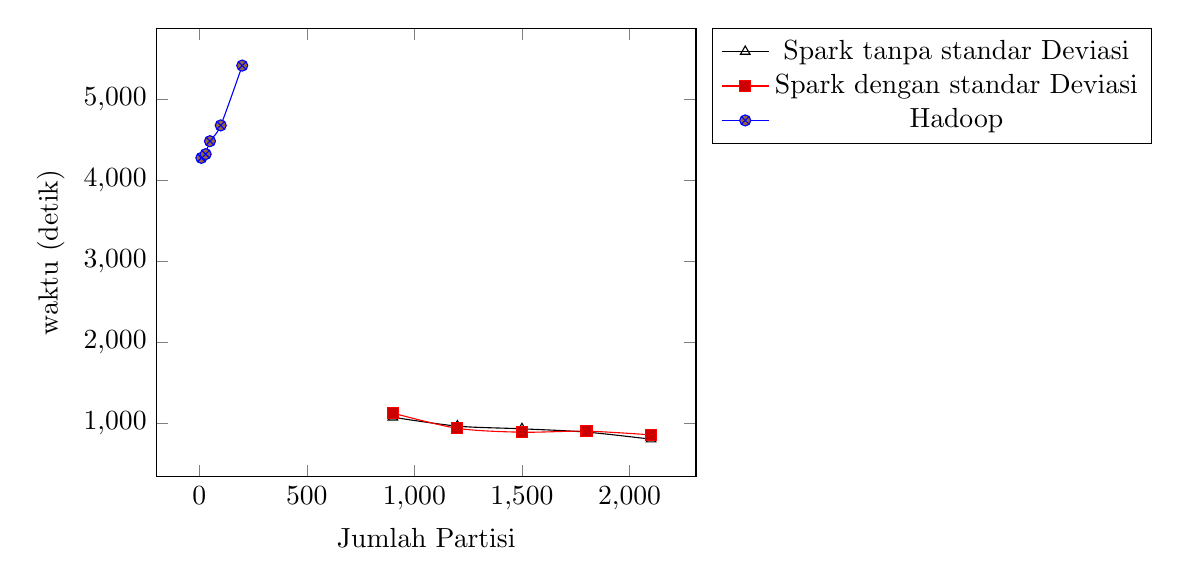
\begin{tikzpicture}[scale=\scl]
		\begin{axis}[\ymin,\ymax,xlabel= Jumlah Partisi,ylabel= waktu (detik), xticklabel style={/pgf/number format/.cd, fixed,fixed zerofill, precision=0},legend pos = outer north east]
		
		\addlegendentry{Spark tanpa standar Deviasi}
		\addplot+[smooth][color=black,mark=triangle] coordinates { (900,1072) (1200,962) (1500,929) (1800,888) (2100,801)};
		\addlegendentry{Spark dengan standar Deviasi}
		\addplot+[smooth][color=red] coordinates { (900,1123) (1200,935) (1500,887) (1800,900) (2100,854)};
		\addlegendentry{Hadoop}
		\addplot+[smooth][color=blue] coordinates {(10,4273) (30,4319) (50,4479) (100,4674) (200,5412) };

		

		\leg
		\end{axis}
		\end{tikzpicture}
		\caption[Hasil Percobaan Jumlah Partisi Spark dan Hadoop dengan Ukuran Data 15 GB, Objek Maksimum 50, dan Total 10 Core]{Hasil Percobaan Jumlah Partisi Spark dan Hadoop dengan Ukuran Data 15 GB, Objek Maksimum 50, dan Total 10 Core}
		\label{fig:percobaan11}
	\end{figure}
\end{minipage}\\



Berdasarkan hasil grafik pada Gambar~\ref{fig:percobaan11}, dapat dilihat waktu Hadoop terus meningkat seiring meningkatnya jumlah partisi. Jumlah partisi yang dicoba pada Hadoop hanya mencapai 200 karena waktu eksekusi yang sudah berbeda jauh dibanding Spark dan untuk partisi yang lebih besar pasti diatas waktu eksekusi Hadoop dengan jumlah partisi sama dengan 200. Spark memiliki waktu eksekusi yang jauh lebih cepat dibanding Hadoop.\\


%%%%%%%%%%%%%%%%%%%%%% MAX OBJ 50 20GB


Percobaan ini menguji waktu eksekusi Spark dan Hadoop berdasarkan jumlah partisi yang optimal. Percobaan ini menggunakan 1 komputer sebagai komputer \textit{master} dan 10 komputer lainya sebagai \textit{worker} dengan setiap \textit{worker} munggunakan 1 core. Ukuran data yang digunakan adalah 20 GB. Metode yang digunakan adalah metode \textit{single linkage} dengan nilai \textit{cut-off distance} adalah 0,8 dan jumlah objek maksimum untuk setiap \textit{dendrogram} adalah 50. Tabel~\ref{tab:spark17} dan Tabel~\ref{tab:spark18} berikut adalah hasil dari eksperimen:





\begin{table}[H] 
	\centering 
	\caption{Percobaan Jumlah Partisi Hadoop dengan Ukuran Data 20 GB}
	\label{tab:spark17}
	\begin{tabular}{|p{3cm}|p{3cm}|p{4cm}|p{4cm}|}
\hline
Ukuran Data (GB) & Jumlah Partisi &  Waktu Eksekusi Hadoop (detik) & Hasil Reduksi Hadoop (GB)\\
\hline
20 & 10 & 5462  & 5.6  \\
\hline
20 & 30 & 5771  & 5.6  \\
\hline
20 & 50 & 5914  & 5.6  \\
\hline
20 & 100 & 6240  & 5.6  \\
\hline
20 & 200 & 7508 & 5.6  \\
\hline


\hline

	\end{tabular} 
\end{table}




\begin{table}[H] 
	\centering 
	\caption{Percobaan Jumlah Partisi Spark dengan Ukuran Data 20 GB}
	\label{tab:spark18}
	\begin{tabular}{|p{1cm}|p{1cm}|p{3cm}|p{3cm}|p{3cm}|p{3cm}|}
\hline
Ukuran Data (GB) & Jumlah Partisi &  Waktu eksekusi Spark Tanpa standar Deviasi (detik) & Waktu Eksekusi Spark (detik) & Hasil Reduksi Spark Tanpa standar Deviasi (GB) & Hasil Reduksi Spark (GB)  \\ 
\hline
20 & 1000 & 1447 &  1546 & 5.6   & 6.9  \\
\hline
20 & 1400 & 1327  & 1242  & 5.6   & 6.9  \\
\hline
20 & 1800 & 1314  & 1278  & 5.6   & 6.9  \\
\hline
20 & 2200 & 1167  & 1246 &  5.6   & 6.9  \\
\hline
20 & 2600 &  1216 &  1220 &  5.6   & 6.9 \\
\hline

\hline

	\end{tabular} 
\end{table}



\def\scl{1}

\def\leg{} 
\def\std{none}
\def\ymin{}
\def\ymax{}

\begin{minipage}[c]{0.9\textwidth}
	\begin{figure}[H]
		\centering
		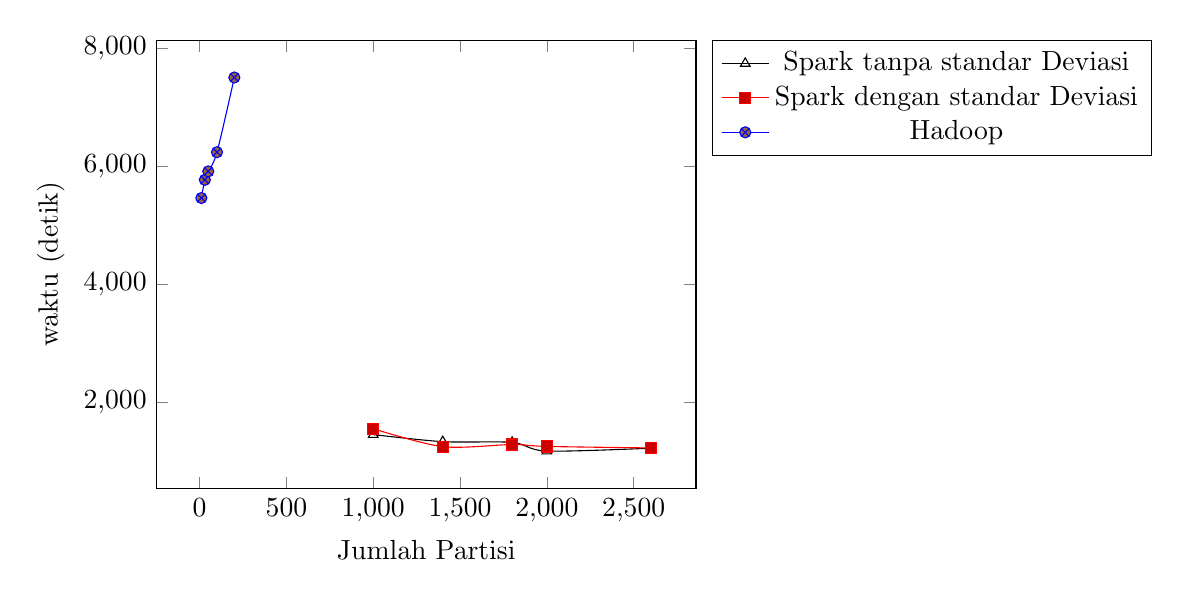
\begin{tikzpicture}[scale=\scl]
		\begin{axis}[\ymin,\ymax,xlabel= Jumlah Partisi,ylabel= waktu (detik), xticklabel style={/pgf/number format/.cd, fixed,fixed zerofill, precision=0},legend pos = outer north east]
		
		\addlegendentry{Spark tanpa standar Deviasi}
		\addplot+[smooth][color=black,mark=triangle] coordinates { (1000,1447) (1400,1327) (1800,1314) (2000,1167) (2600,1216)};
		\addlegendentry{Spark dengan standar Deviasi}
		\addplot+[smooth][color=red] coordinates { (1000,1546) (1400,1242) (1800,1278) (2000,1246) (2600,1220)};
		\addlegendentry{Hadoop}
		\addplot+[smooth][color=blue] coordinates {(10,5462) (30,5771) (50,5914) (100,6240) (200,7508) };

		

		\leg
		\end{axis}
		\end{tikzpicture}
		\caption[Hasil Percobaan Jumlah Partisi Spark dan Hadoop dengan Ukuran Data 20 GB, Objek Maksimum 50, dan Total 10 Core]{Hasil Percobaan Jumlah Partisi Spark dan Hadoop dengan Ukuran Data 20 GB, Objek Maksimum 50, dan Total 10 Core}
		\label{fig:percobaan12}
	\end{figure}
\end{minipage}\\



Berdasarkan hasil grafik pada Gambar~\ref{fig:percobaan12}, dapat dilihat waktu Hadoop terus meningkat seiring meningkatnya jumlah partisi. Jumlah partisi yang dicoba pada Hadoop hanya mencapai 200 karena waktu eksekusi yang sudah berbeda jauh dibanding Spark dan untuk partisi yang lebih besar pasti diatas waktu eksekusi Hadoop dengan jumlah partisi sama dengan 200. Spark memiliki waktu eksekusi yang jauh lebih cepat dibanding Hadoop. \\








%%%%%%%%%%%%%%%%%%%%%%%%%%%%%%% MAX OBJ 100



%%%%%%%%%%%%%%%% MAX OBJ 100



%%%%%%%%%%%%%%%%%%%%%%%%%%%%%%%%%%% MAX OBJ 100 5 GB

Percobaan ini menguji waktu eksekusi Spark dan Hadoop berdasarkan jumlah partisi yang optimal. Percobaan ini menggunakan 1 komputer sebagai komputer \textit{master} dan 10 komputer lainya sebagai \textit{worker} dengan setiap \textit{worker} munggunakan 1 core. Ukuran data yang digunakan adalah 5 GB. Metode yang digunakan adalah metode \textit{single linkage} dengan nilai \textit{cut-off distance} adalah 0,8 dan jumlah objek maksimum untuk setiap \textit{dendrogram} adalah 100. Tabel~\ref{tab:spark111} dan Tabel~\ref{tab:spark121} berikut adalah hasil dari eksperimen:





\begin{table}[H] 
	\centering 
	\caption{Percobaan Jumlah Partisi Hadoop dengan Ukuran Data 5 GB}
	\label{tab:spark111}
	\begin{tabular}{|p{3cm}|p{3cm}|p{4cm}|p{4cm}|}
\hline
Ukuran Data (GB) & Jumlah Partisi &  Waktu Eksekusi Hadoop (menit) & Hasil Reduksi Hadoop (GB)\\
\hline
5 & 10 & 101  & 0.962  \\
\hline
5 & 30 & 103  & 0.962  \\
\hline
5 & 50 & 106  & 0.962   \\
\hline


\hline

	\end{tabular} 
\end{table}






\begin{table}[H] 
	\centering 
	\caption{Percobaan Jumlah Partisi Spark dengan Ukuran Data 5 GB}
	\label{tab:spark121}
	\begin{tabular}{|p{1cm}|p{1cm}|p{3cm}|p{3cm}|p{3cm}|p{3cm}|}
\hline
Ukuran Data (GB) & Jumlah Partisi &  Waktu eksekusi Spark Tanpa standar Deviasi (menit) & Waktu Eksekusi Spark (menit) & Hasil Reduksi Spark Tanpa standar Deviasi (GB) & Hasil Reduksi Spark (GB)  \\ 
\hline
5 & 300 & 6.9 &  7.5 & 1  & 1.2 \\
\hline
5 & 400 & 6.8  & 7.0  & 1  & 1.2 \\
\hline
5 & 500 & 6.7  & 6.7  & 1  & 1.2 \\
\hline
5 & 600 & 6.5  & 6.8 &  1  & 1.2 \\
\hline
5 & 700 & 6.4  &  6.3 &  1  & 1.2 \\
\hline

\hline

	\end{tabular} 
\end{table}



\def\scl{1}

\def\leg{} 
\def\std{none}
\def\ymin{}
\def\ymax{}

\begin{minipage}[c]{0.9\textwidth}
	\begin{figure}[H]
		\centering
		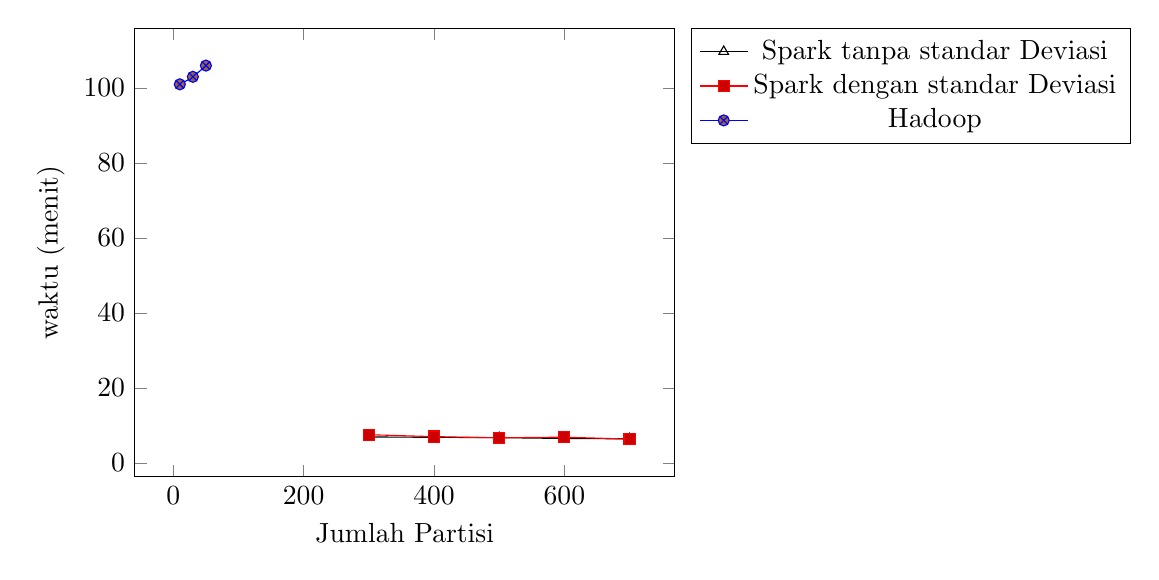
\begin{tikzpicture}[scale=\scl]
		\begin{axis}[\ymin,\ymax,xlabel= Jumlah Partisi,ylabel= waktu (menit), xticklabel style={/pgf/number format/.cd, fixed,fixed zerofill, precision=0},legend pos = outer north east]
		
		\addlegendentry{Spark tanpa standar Deviasi}
		\addplot+[smooth][color=black,mark=triangle] coordinates { (300,6.9) (400,6.8) (500,6.7) (600,6.5) (700,6.4)};
		\addlegendentry{Spark dengan standar Deviasi}
		\addplot+[smooth][color=red] coordinates { (300,7.5) (400,7.0) (500,6.7) (600,6.8) (700,6.3)};
		\addlegendentry{Hadoop}
		\addplot+[smooth][color=blue] coordinates {(10,101) (30,103) (50,106)};


		

		\leg
		\end{axis}
		\end{tikzpicture}
		\caption[Hasil Percobaan Jumlah Partisi Spark dan Hadoop dengan Ukuran Data 5 GB, Objek Maksimum 100, dan Total 10 Core]{Hasil Percobaan Jumlah Partisi Spark dan Hadoop dengan Ukuran Data 5 GB, Objek Maksimum 100, dan Total 10 Core}
		\label{fig:percobaan91}
	\end{figure}
\end{minipage}\\



Berdasarkan hasil grafik pada Gambar~\ref{fig:percobaan91}, dapat dilihat waktu Hadoop terus meningkat seiring meningkatnya jumlah partisi. Jumlah partisi yang dicoba pada Hadoop hanya mencapai 200 karena waktu eksekusi yang sudah berbeda jauh dibanding Spark dan untuk partisi yang lebih besar pasti diatas waktu eksekusi Hadoop dengan jumlah partisi sama dengan 200. Spark memiliki waktu eksekusi yang jauh lebih cepat dibanding Hadoop.  \\

%%%%%%%%%%%%%%%%%%%%%%%%%%%%%%%%%%% MAX OBJ 100 10 GB


Percobaan ini menguji waktu eksekusi Spark dan Hadoop berdasarkan jumlah partisi yang optimal. Percobaan ini menggunakan 1 komputer sebagai komputer \textit{master} dan 10 komputer lainya sebagai \textit{worker} dengan setiap \textit{worker} munggunakan 1 core. Ukuran data yang digunakan adalah 10 GB. Metode yang digunakan adalah metode \textit{single linkage} dengan nilai \textit{cut-off distance} adalah 0,8 dan jumlah objek maksimum untuk setiap \textit{dendrogram} adalah 100. Tabel~\ref{tab:spark131} dan Tabel~\ref{tab:spark141} berikut adalah hasil dari eksperimen:





\begin{table}[H] 
	\centering 
	\caption{Percobaan Jumlah Partisi Hadoop dengan Ukuran Data 10 GB}
	\label{tab:spark131}
	\begin{tabular}{|p{3cm}|p{3cm}|p{4cm}|p{4cm}|}
\hline
Ukuran Data (GB) & Jumlah Partisi &  Waktu Eksekusi Hadoop (menit) & Hasil Reduksi Hadoop (GB)\\
\hline
10 & 10 & 181  & 1.7  \\
\hline
10 & 30 & 182  & 1.7  \\
\hline
10 & 50 & 184  & 1.7   \\
\hline


\hline

	\end{tabular} 
\end{table}




\begin{table}[H] 
	\centering 
	\caption{Percobaan Jumlah Partisi Spark dengan Ukuran Data 10 GB}
	\label{tab:spark141}
	\begin{tabular}{|p{1cm}|p{1cm}|p{3cm}|p{3cm}|p{3cm}|p{3cm}|}
\hline
Ukuran Data (GB) & Jumlah Partisi &  Waktu eksekusi Spark Tanpa standar Deviasi (menit) & Waktu Eksekusi Spark (menit) & Hasil Reduksi Spark Tanpa standar Deviasi (GB) & Hasil Reduksi Spark (GB)  \\ 
\hline
10 & 500 &  12.5  &  12.4  & 1.8  & 2.2  \\
\hline
10 & 700 & 11.5  & 12.0  & 1.8  & 2.2  \\
\hline
10 & 900 & 12.2  & 11.6  & 1.8  & 2.2  \\
\hline
10 & 1100 & 11.5  &  11.0 &  1.8 & 2.2  \\
\hline
10 & 1300 &  10.6 &  11.2 &  1.8  & 2.2  \\
\hline

\hline

	\end{tabular} 
\end{table}



\def\scl{1}

\def\leg{} 
\def\std{none}
\def\ymin{}
\def\ymax{}

\begin{minipage}[c]{0.9\textwidth}
	\begin{figure}[H]
		\centering
		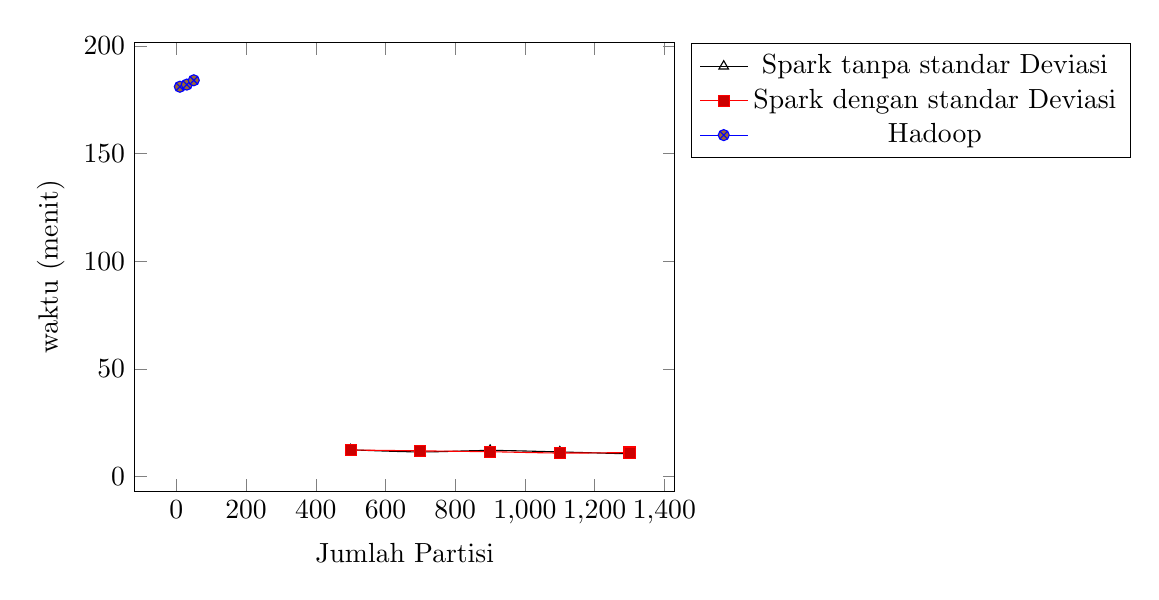
\begin{tikzpicture}[scale=\scl]
		\begin{axis}[\ymin,\ymax,xlabel= Jumlah Partisi,ylabel= waktu (menit), xticklabel style={/pgf/number format/.cd, fixed,fixed zerofill, precision=0},legend pos = outer north east]
		
		\addlegendentry{Spark tanpa standar Deviasi}
		\addplot+[smooth][color=black,mark=triangle] coordinates { (500,12.5) (700,11.5) (900,12.2) (1100,11.5) (1300,10.6)};
		\addlegendentry{Spark dengan standar Deviasi}
		\addplot+[smooth][color=red] coordinates { (500,12.4) (700,12.0) (900,11.6) (1100,11.0) (1300,11.2)};
		\addlegendentry{Hadoop}
		\addplot+[smooth][color=blue] coordinates {(10,181) (30,182) (50,184)  };

		

		\leg
		\end{axis}
		\end{tikzpicture}
		\caption[Hasil Percobaan Jumlah Partisi Spark dan Hadoop dengan Ukuran Data 10 GB, Objek Maksimum 100, dan Total 10 Core]{Hasil Percobaan Jumlah Partisi Spark dan Hadoop dengan Ukuran Data 10 GB, Objek Maksimum 100, dan Total 10 Core}
		\label{fig:percobaan101}
	\end{figure}
\end{minipage}\\



Berdasarkan hasil grafik pada Gambar~\ref{fig:percobaan101}, dapat dilihat waktu Hadoop terus meningkat seiring meningkatnya jumlah partisi. Jumlah partisi yang dicoba pada Hadoop hanya mencapai 200 karena waktu eksekusi yang sudah berbeda jauh dibanding Spark dan untuk partisi yang lebih besar pasti diatas waktu eksekusi Hadoop dengan jumlah partisi sama dengan 200. Spark memiliki waktu eksekusi yang jauh lebih cepat dibanding Hadoop.  \\



%%%%%%%%%%%%%%%%%%%%%%%%%%%%%%%%%%% MAX OBJ 100 15 GB


Percobaan ini menguji waktu eksekusi Spark dan Hadoop berdasarkan jumlah partisi yang optimal. Percobaan ini menggunakan 1 komputer sebagai komputer \textit{master} dan 10 komputer lainya sebagai \textit{worker} dengan setiap \textit{worker} munggunakan 1 core. Ukuran data yang digunakan adalah 15 GB. Metode yang digunakan adalah metode \textit{single linkage} dengan nilai \textit{cut-off distance} adalah 0,8 dan jumlah objek maksimum untuk setiap \textit{dendrogram} adalah 100. Tabel~\ref{tab:spark151} dan Tabel~\ref{tab:spark161} berikut adalah hasil dari eksperimen:





\begin{table}[H] 
	\centering 
	\caption{Percobaan Jumlah Partisi Hadoop dengan Ukuran Data 15 GB}
	\label{tab:spark151}
	\begin{tabular}{|p{3cm}|p{3cm}|p{4cm}|p{4cm}|}
\hline
Ukuran Data (GB) & Jumlah Partisi &  Waktu Eksekusi Hadoop (menit) & Hasil Reduksi Hadoop (GB)\\
\hline
15 & 10 & 270  & 2.6  \\
\hline
15 & 30 & 266  & 2.6  \\
\hline
15 & 50 & 275  & 2.6  \\
\hline


\hline

	\end{tabular} 
\end{table}




\begin{table}[H] 
	\centering 
	\caption{Percobaan Jumlah Partisi Spark dengan Ukuran Data 15 GB}
	\label{tab:spark161}
	\begin{tabular}{|p{1cm}|p{1cm}|p{3cm}|p{3cm}|p{3cm}|p{3cm}|}
\hline
Ukuran Data (GB) & Jumlah Partisi &  Waktu eksekusi Spark Tanpa standar Deviasi (menit) & Waktu Eksekusi Spark (menit) & Hasil Reduksi Spark Tanpa standar Deviasi (GB) & Hasil Reduksi Spark (GB)  \\ 
\hline
15 & 900 &  18.0 &  18.6 & 2.8  & 3.4 \\
\hline
15 & 1200 & 18.5  & 18.4  & 2.8  & 3.4 \\
\hline
15 & 1500 & 17.3  & 16.3  & 2.8  & 3.4 \\
\hline
15 & 1800 & 17.4  & 17.6 &  2.8  & 3.4 \\
\hline
15 & 2100 & 17.3 &  17.7 &  2.8 & 3.4 \\
\hline

\hline

	\end{tabular} 
\end{table}



\def\scl{1}

\def\leg{} 
\def\std{none}
\def\ymin{}
\def\ymax{}

\begin{minipage}[c]{0.9\textwidth}
	\begin{figure}[H]
		\centering
		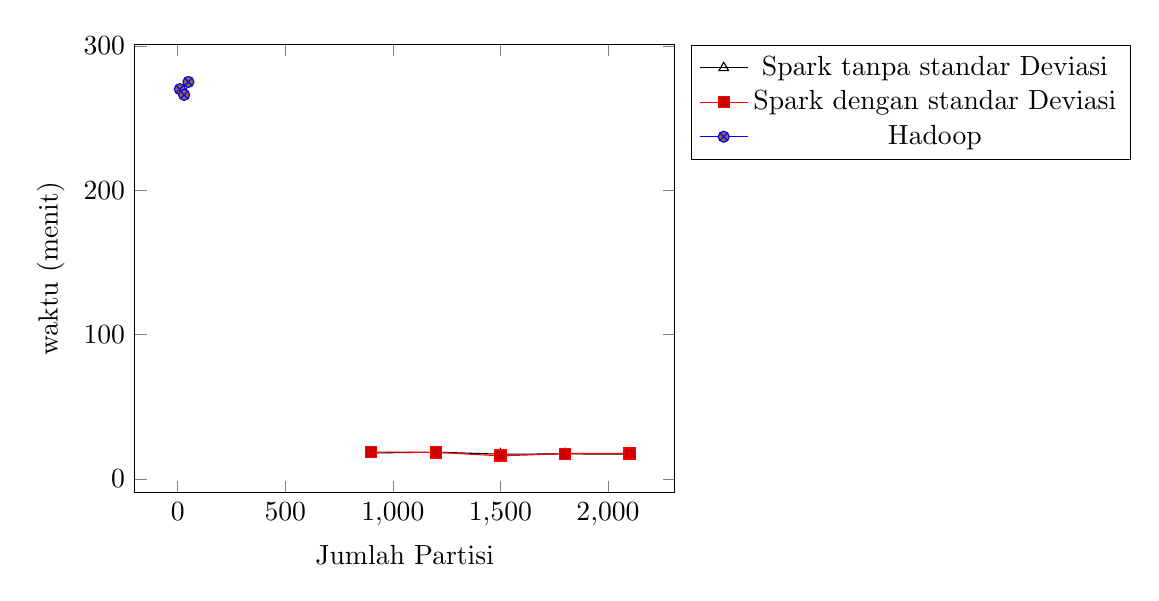
\begin{tikzpicture}[scale=\scl]
		\begin{axis}[\ymin,\ymax,xlabel= Jumlah Partisi,ylabel= waktu (menit), xticklabel style={/pgf/number format/.cd, fixed,fixed zerofill, precision=0},legend pos = outer north east]
		
		\addlegendentry{Spark tanpa standar Deviasi}
		\addplot+[smooth][color=black,mark=triangle] coordinates { (900,18.0) (1200,18.5) (1500,17.3) (1800,17.4) (2100,17.3)};
		\addlegendentry{Spark dengan standar Deviasi}
		\addplot+[smooth][color=red] coordinates { (900,18.6) (1200,18.4) (1500,16.3) (1800,17.6) (2100,17.7)};
		\addlegendentry{Hadoop}
		\addplot+[smooth][color=blue] coordinates {(10,270) (30,266) (50,275) };

		

		\leg
		\end{axis}
		\end{tikzpicture}
		\caption[Hasil Percobaan Jumlah Partisi Spark dan Hadoop dengan Ukuran Data 15 GB, Objek Maksimum 100, dan Total 10 Core]{Hasil Percobaan Jumlah Partisi Spark dan Hadoop dengan Ukuran Data 15 GB, Objek Maksimum 100, dan Total 10 Core}
		\label{fig:percobaan111}
	\end{figure}
\end{minipage}\\



Berdasarkan hasil grafik pada Gambar~\ref{fig:percobaan111}, dapat dilihat waktu Hadoop terus meningkat seiring meningkatnya jumlah partisi. Jumlah partisi yang dicoba pada Hadoop hanya mencapai 200 karena waktu eksekusi yang sudah berbeda jauh dibanding Spark dan untuk partisi yang lebih besar pasti diatas waktu eksekusi Hadoop dengan jumlah partisi sama dengan 200. Spark memiliki waktu eksekusi yang jauh lebih cepat dibanding Hadoop. \\


%%%%%%%%%%%%%%%%%%%%%%  MAX OBJ 100 20GB


Percobaan ini menguji waktu eksekusi Spark dan Hadoop berdasarkan jumlah partisi yang optimal. Percobaan ini menggunakan 1 komputer sebagai komputer \textit{master} dan 10 komputer lainya sebagai \textit{worker} dengan setiap \textit{worker} munggunakan 1 core. Ukuran data yang digunakan adalah 20 GB. Metode yang digunakan adalah metode \textit{single linkage} dengan nilai \textit{cut-off distance} adalah 0,8 dan jumlah objek maksimum untuk setiap \textit{dendrogram} adalah 100. Tabel~\ref{tab:spark171} dan Tabel~\ref{tab:spark181} berikut adalah hasil dari eksperimen:





\begin{table}[H] 
	\centering 
	\caption{Percobaan Jumlah Partisi Hadoop dengan Ukuran Data 20 GB}
	\label{tab:spark171}
	\begin{tabular}{|p{3cm}|p{3cm}|p{4cm}|p{4cm}|}
\hline
Ukuran Data (GB) & Jumlah Partisi &  Waktu Eksekusi Hadoop (menit) & Hasil Reduksi Hadoop (GB)\\
\hline
20 & 10 & 350  & 3.5  \\
\hline
20 & 30 & 358  & 3.5  \\
\hline
20 & 50 & 365  & 3.5  \\
\hline


\hline

	\end{tabular} 
\end{table}




\begin{table}[H] 
	\centering 
	\caption{Percobaan Jumlah Partisi Spark dengan Ukuran Data 20 GB}
	\label{tab:spark181}
	\begin{tabular}{|p{1cm}|p{1cm}|p{3cm}|p{3cm}|p{3cm}|p{3cm}|}
\hline
Ukuran Data (GB) & Jumlah Partisi &  Waktu eksekusi Spark Tanpa standar Deviasi (menit) & Waktu Eksekusi Spark (menit) & Hasil Reduksi Spark Tanpa standar Deviasi (GB) & Hasil Reduksi Spark (GB)  \\ 
\hline
20 & 1000 & 24.7  &  25.7 & 3.7   & 4.5  \\
\hline
20 & 1400 & 24.3  & 23.5  & 3.7   & 4.5  \\
\hline
20 & 1800 & 24.0  & 23.4  & 3.7   & 4.5  \\
\hline
20 & 2200 & 24.2  & 23.2 &  3.7   & 4.5  \\
\hline
20 & 2600 & 23.8 &  23.7 &  3.7  & 4.5 \\
\hline

\hline

	\end{tabular} 
\end{table}



\def\scl{1}

\def\leg{} 
\def\std{none}
\def\ymin{}
\def\ymax{}

\begin{minipage}[c]{0.9\textwidth}
	\begin{figure}[H]
		\centering
		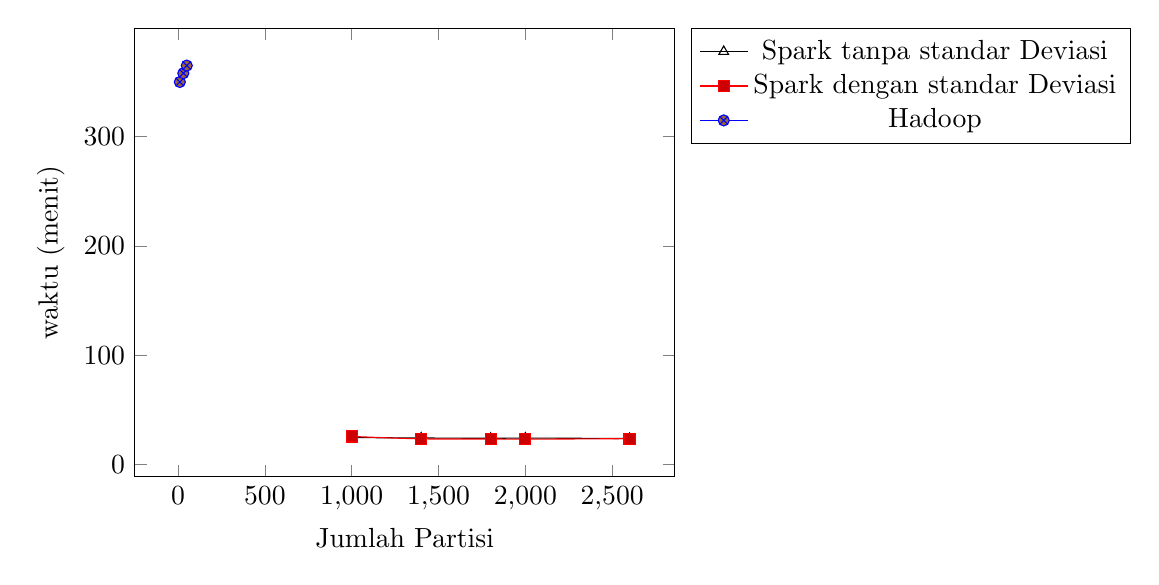
\begin{tikzpicture}[scale=\scl]
		\begin{axis}[\ymin,\ymax,xlabel= Jumlah Partisi,ylabel= waktu (menit), xticklabel style={/pgf/number format/.cd, fixed,fixed zerofill, precision=0},legend pos = outer north east]
		
		\addlegendentry{Spark tanpa standar Deviasi}
		\addplot+[smooth][color=black,mark=triangle] coordinates { (1000,24.7) (1400,24.3) (1800,24.0) (2000,24.2) (2600,23.8)};
		\addlegendentry{Spark dengan standar Deviasi}
		\addplot+[smooth][color=red] coordinates { (1000,25.7) (1400,23.5) (1800,23.4) (2000,23.2) (2600,23.7)};
		\addlegendentry{Hadoop}
		\addplot+[smooth][color=blue] coordinates {(10,350) (30,358) (50,365)};

		

		\leg
		\end{axis}
		\end{tikzpicture}
		\caption[Hasil Percobaan Jumlah Partisi Spark dan Hadoop dengan Ukuran Data 20 GB, Objek Maksimum 100, dan Total 10 Core]{Hasil Percobaan Jumlah Partisi Spark dan Hadoop dengan Ukuran Data 20 GB, Objek Maksimum 100, dan Total 10 Core}
		\label{fig:percobaan121}
	\end{figure}
\end{minipage}\\



Berdasarkan hasil grafik pada Gambar~\ref{fig:percobaan121}, dapat dilihat waktu Hadoop terus meningkat seiring meningkatnya jumlah partisi. Jumlah partisi yang dicoba pada Hadoop hanya mencapai 200 karena waktu eksekusi yang sudah berbeda jauh dibanding Spark dan untuk partisi yang lebih besar pasti diatas waktu eksekusi Hadoop dengan jumlah partisi sama dengan 200. Spark memiliki waktu eksekusi yang jauh lebih cepat dibanding Hadoop. \\

















%%%%%%%%%%%%%%%%%%% COMPLETE LINKAGE


Percobaan ini menguji waktu eksekusi Spark dan Hadoop berdasarkan jumlah partisi yang optimal. Percobaan ini menggunakan 1 komputer sebagai komputer \textit{master} dan 10 komputer lainya sebagai \textit{worker} dengan setiap \textit{worker} munggunakan 1 core. Ukuran data yang digunakan adalah 10 GB. Metode yang digunakan adalah metode \textit{complete linkage} dengan nilai \textit{cut-off distance} adalah 0,8 dan jumlah objek maksimum untuk setiap \textit{dendrogram} adalah 30. Tabel~\ref{tab:spark571} dan Tabel~\ref{tab:spark581} berikut adalah hasil dari eksperimen:


\begin{table}[H] 
	\centering 
	\caption{Percobaan Jumlah Partisi Hadoop dengan Ukuran Data 10 GB}
	\label{tab:spark571}
	\begin{tabular}{|p{3cm}|p{3cm}|p{4cm}|p{4cm}|}
\hline
Ukuran Data (GB) & Jumlah Partisi &  Waktu Eksekusi Hadoop (detik) & Hasil Reduksi Hadoop (GB)\\
\hline
10 & 10 & 1510  & 2.4  \\
\hline
10 & 30 & 1592  & 2.4  \\
\hline
10 & 50 & 1600  & 2.4  \\
\hline
10 & 100 & 1841  & 2.4  \\
\hline
10 & 200 & 2787  & 2.4  \\
\hline

\hline

	\end{tabular} 
\end{table}




\begin{table}[H] 
	\centering 
	\caption{Percobaan Jumlah Partisi Spark dengan Ukuran Data 10 GB}
	\label{tab:spark581}
	\begin{tabular}{|p{1cm}|p{1cm}|p{3cm}|p{3cm}|p{3cm}|p{3cm}|}
\hline
Ukuran Data (GB) & Jumlah Partisi &  Waktu eksekusi Spark Tanpa standar Deviasi (detik) & Waktu Eksekusi Spark (detik) & Hasil Reduksi Spark Tanpa standar Deviasi (GB) & Hasil Reduksi Spark (GB)  \\ 
\hline
10 & 500 &  643  &  664  & 2.3  & 3.0  \\
\hline
10 & 700 & 465  & 523  & 2.3  & 3.0  \\
\hline
10 & 900 & 438  & 463  & 2.3  & 3.0  \\
\hline
10 & 1100 & 405  &  413 &  2.3 & 3.0  \\
\hline
10 & 1300 & 398 &  394 &  2.3  & 3.0  \\
\hline
\hline


	\end{tabular} 
\end{table}


\def\scl{1}

\def\leg{} 
\def\std{none}
\def\ymin{}
\def\ymax{}

\begin{minipage}[c]{0.9\textwidth}
	\begin{figure}[H]
		\centering
		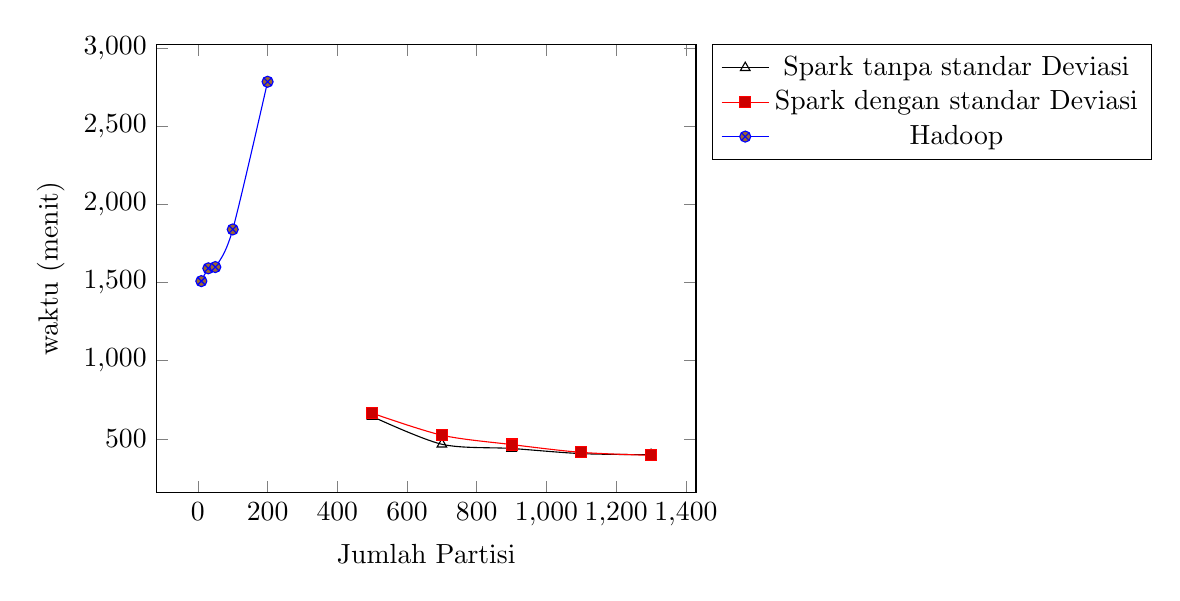
\begin{tikzpicture}[scale=\scl]
		\begin{axis}[\ymin,\ymax,xlabel= Jumlah Partisi,ylabel= waktu (menit), xticklabel style={/pgf/number format/.cd, fixed,fixed zerofill, precision=0},legend pos = outer north east]
		
		\addlegendentry{Spark tanpa standar Deviasi}
		\addplot+[smooth][color=black,mark=triangle] coordinates { (500,643) (700,465) (900,438) (1100,405) (1300,398)};
		\addlegendentry{Spark dengan standar Deviasi}
		\addplot+[smooth][color=red] coordinates { (500,664) (700,523) (900,463) (1100,413) (1300,394)};
		\addlegendentry{Hadoop}
		\addplot+[smooth][color=blue] coordinates {(10,1510) (30,1592) (50,1600) (100,1841) (200,2787)};

		

		\leg
		\end{axis}
		\end{tikzpicture}
		\caption[Hasil Percobaan Jumlah Partisi Spark dan Hadoop dengan Ukuran Data 10 GB, Objek Maksimum 30, dan Total 10 Core]{Hasil Percobaan Jumlah Partisi Spark dan Hadoop dengan Ukuran Data 20 GB, Objek Maksimum 30, dan Total 10 Core}
		\label{fig:percobaan521}
	\end{figure}
\end{minipage}\\



Berdasarkan hasil grafik pada Gambar~\ref{fig:percobaan521}, dapat dilihat waktu Hadoop terus meningkat seiring meningkatnya jumlah partisi. Jumlah partisi yang dicoba pada Hadoop hanya mencapai 200 karena waktu eksekusi yang sudah berbeda jauh dibanding Spark dan untuk partisi yang lebih besar pasti diatas waktu eksekusi Hadoop dengan jumlah partisi sama dengan 200. Spark memiliki waktu eksekusi yang jauh lebih cepat dibanding Hadoop. \\




%%%%%%%%%%%%%%%%%%%% CENTROID LINKAGE



Percobaan ini menguji waktu eksekusi Spark dan Hadoop berdasarkan jumlah partisi yang optimal. Percobaan ini menggunakan 1 komputer sebagai komputer \textit{master} dan 10 komputer lainya sebagai \textit{worker} dengan setiap \textit{worker} munggunakan 1 core. Ukuran data yang digunakan adalah 10 GB. Metode yang digunakan adalah metode \textit{centroid linkage}, dengan nilai \textit{cut-off distance} adalah 0,8 dan jumlah objek maksimum untuk setiap \textit{dendrogram} adalah 30. Tabel~\ref{tab:spark671} dan Tabel~\ref{tab:spark681} berikut adalah hasil dari eksperimen:


\begin{table}[H] 
	\centering 
	\caption{Percobaan Jumlah Partisi Hadoop dengan Ukuran Data 10 GB}
	\label{tab:spark671}
	\begin{tabular}{|p{3cm}|p{3cm}|p{4cm}|p{4cm}|}
\hline
Ukuran Data (GB) & Jumlah Partisi &  Waktu Eksekusi Hadoop (detik) & Hasil Reduksi Hadoop (GB)\\
\hline
10 & 10 & 986  & 2.7  \\
\hline
10 & 30 & 1073  & 2.7  \\
\hline
10 & 50 & 1116  & 2.7  \\
\hline
10 & 100 & 1294  & 2.7  \\
\hline
10 & 200 & 1720  & 2.7  \\
\hline

\hline

	\end{tabular} 
\end{table}




\begin{table}[H] 
	\centering 
	\caption{Percobaan Jumlah Partisi Spark dengan Ukuran Data 10 GB}
	\label{tab:spark681}
	\begin{tabular}{|p{1cm}|p{1cm}|p{3cm}|p{3cm}|p{3cm}|p{3cm}|}
\hline
Ukuran Data (GB) & Jumlah Partisi &  Waktu eksekusi Spark Tanpa standar Deviasi (detik) & Waktu Eksekusi Spark (detik) & Hasil Reduksi Spark Tanpa standar Deviasi (GB) & Hasil Reduksi Spark (GB)  \\ 
\hline
10 & 500 & 589  &  604  & 2.8  & 3.7  \\
\hline
10 & 700 & 597  & 600  & 2.8  & 3.7  \\
\hline
10 & 900 & 469  & 533  & 2.8  & 3.7  \\
\hline
10 & 1100 & 458  & 491 &  2.8 & 3.7  \\
\hline
10 & 1300 & 438 &  438 &  2.8  & 3.7  \\
\hline
\hline


	\end{tabular} 
\end{table}


\def\scl{1}

\def\leg{} 
\def\std{none}
\def\ymin{}
\def\ymax{}

\begin{minipage}[c]{0.9\textwidth}
	\begin{figure}[H]
		\centering
		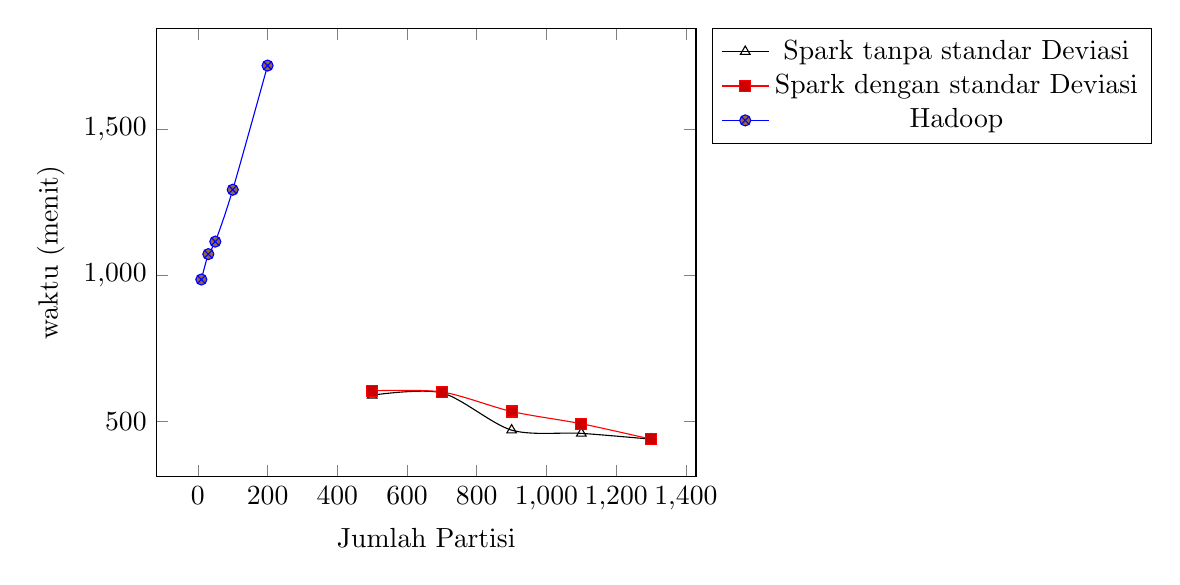
\begin{tikzpicture}[scale=\scl]
		\begin{axis}[\ymin,\ymax,xlabel= Jumlah Partisi,ylabel= waktu (menit), xticklabel style={/pgf/number format/.cd, fixed,fixed zerofill, precision=0},legend pos = outer north east]
		
		\addlegendentry{Spark tanpa standar Deviasi}
		\addplot+[smooth][color=black,mark=triangle] coordinates { (500,589) (700,597) (900,469) (1100,458) (1300,438)};
		\addlegendentry{Spark dengan standar Deviasi}
		\addplot+[smooth][color=red] coordinates { (500,604) (700,600) (900,533) (1100,491) (1300,438)};
		\addlegendentry{Hadoop}
		\addplot+[smooth][color=blue] coordinates {(10,986) (30,1073) (50,1116) (100,1294) (200,1720)};

		

		\leg
		\end{axis}
		\end{tikzpicture}
		\caption[Hasil Percobaan Jumlah Partisi Spark dan Hadoop dengan Ukuran Data 10 GB, Objek Maksimum 30, dan Total 10 Core]{Hasil Percobaan Jumlah Partisi Spark dan Hadoop dengan Ukuran Data 20 GB, Objek Maksimum 30, dan Total 10 Core}
		\label{fig:percobaan621}
	\end{figure}
\end{minipage}\\



Berdasarkan hasil grafik pada Gambar~\ref{fig:percobaan621}, dapat dilihat waktu Hadoop terus meningkat seiring meningkatnya jumlah partisi. Jumlah partisi yang dicoba pada Hadoop hanya mencapai 200 karena waktu eksekusi yang sudah berbeda jauh dibanding Spark dan untuk partisi yang lebih besar pasti diatas waktu eksekusi Hadoop dengan jumlah partisi sama dengan 200. Spark memiliki waktu eksekusi yang jauh lebih cepat dibanding Hadoop. \\


Berdasarkan eksperimen-eksperimen diatas, dapat disimpulkan bahwa Spark dapat bekerja lebih cepat dibanding Hadoop pada partisi yang besar. Sebaliknya, waktu eksekusi Hadoop meningkat ketika jumlah partisi ditingkatkan. Waktu eksekusi Hadoop terbaik dapat masih lebih tinggi dibanding waktu eksekusi terbaik Spark. Meningkatnya waktu eksekusi Hadoop disebabkan oleh \textit{shuffling} dan \textit{sorting}. Semakin tinggi jumlah partisi, semakin banyak yang di-\textit{shuffle} dan di-\textit{sorting}. Berbeda dengan Hadoop, waktu eksekusi Spark menurun ketika jumlah partisi ditingkatkan. Dengan meningkatkan jumlah partisi pada Spark, data akan lebih terdistribusi. Hal ini akan mengurangi waktu yang dibutuhkan untuk mengirim data dari satu komputer ke komputer lain dan mengurangi waktu komunikasi.